\documentclass[11pt,a4paper]{article}

\usepackage[margin=1in, paperwidth=8.3in, paperheight=11.7in]{geometry}
\usepackage{amsfonts}
\usepackage{amsmath}
\usepackage{dsfont}
\usepackage{enumerate}
\usepackage{enumitem}
\usepackage{fancyhdr}
\usepackage{graphicx}
\usepackage{tikz}
\usetikzlibrary{automata,positioning}

\begin{document}

\pagestyle{fancy}
\setlength\parindent{0pt}
\allowdisplaybreaks

\renewcommand{\headrulewidth}{0pt}

% Cover page title
\title{Probability 2 - Notes}
\author{Dom Hutchinson}
\date{\today}
\maketitle

% Header
\fancyhead[L]{Dom Hutchinson}
\fancyhead[C]{Probability 2 - Notes}
\fancyhead[R]{\today}

% enumerate uses roman
\setlist[enumerate,1]{label=\roman*)}

% Counters
\newcounter{definition}[section]
\newcounter{example}[section]
\newcounter{notation}[section]
\newcounter{proof}[section]
\newcounter{proposition}[section]
\newcounter{remark}[section]
\newcounter{theorem}[section]

% commands
\newcommand{\dotprod}[0]{\boldsymbol{\cdot}}
\newcommand{\cosech}[0]{\mathrm{cosech}\ }
\newcommand{\cosec}[0]{\mathrm{cosec}\ }
\newcommand{\sech}[0]{\mathrm{sech}\ }
\newcommand{\expect}[0]{\mathbb{E}}
\newcommand{\nats}[0]{\mathbb{N}}
\newcommand{\prob}[0]{\mathbb{P}}
\newcommand{\real}[0]{\mathbb{R}}
\newcommand{\sigmafield}[0]{\mathcal{F}}
\newcommand{\nb}[0]{\textit{N.B. }}

\newcommand{\definition}[1]{\stepcounter{definition} \textbf{Definition \arabic{section}.\arabic{definition}\ - }\textit{#1}\\}
\newcommand{\example}[1]{\stepcounter{example} \textbf{Example \arabic{section}.\arabic{example}\ - }\textit{#1}\\}
\newcommand{\notation}[1]{\stepcounter{notation} \textbf{Notation \arabic{section}.\arabic{notation}\ - }\textit{#1}\\}
\newcommand{\proof}[1]{\stepcounter{proof} \textbf{Proof \arabic{section}.\arabic{proof}\ - }\textit{#1}\\}
\newcommand{\Proof}[1]{\stepcounter{proof} \textbf{Proof \arabic{section}.\arabic{proof}\ - }\textit{#1}}
\newcommand{\proposition}[1]{\stepcounter{proposition} \textbf{Proposition \arabic{section}.\arabic{proposition}\ - }\textit{#1}\\}
\newcommand{\remark}[1]{\stepcounter{remark} \textbf{Remark \arabic{section}.\arabic{remark}\ - }\textit{#1}\\}
\newcommand{\theorem}[1]{\stepcounter{theorem} \textbf{Theorem \arabic{section}.\arabic{theorem}\ - }\textit{#1}\\}

\tableofcontents

% Start of content
\newpage

\section{Introduction}

\subsection{The Probability Triple}

\definition{Sample Space, $\Omega$}
A \textit{Sample Space}, $\Omega$, is the set of all possible outcomes.\\

\definition{Sigma Field, $\sigma-Field$}
A \textit{Sigma Field}, $\sigmafield$, of subsets of a sample space $\Omega$ satisfies the following conditions
\begin{enumerate}[label=\roman*)]
	\item $\emptyset\in\sigmafield$;
	\item If $A_1,A_2,\dots\in\sigmafield$ then $\bigcup\limits_{i=1}^\infty A_i\in\sigmafield$; And,
	\item If $A\in\sigmafield$ then $A^c\in\sigmafield$ where $A^c:=\Omega\backslash A$.
\end{enumerate}

\definition{Probability Space}
A \textit{Probability Space} is a triple $(\Omega,\sigmafield,\prob)$.

\subsection{The Sigma Field}

\definition{$\sigmafield$-measurable}
Events in $\sigmafield$ are said to be $\sigmafield$-measurable.\\
If an event $A$ is $\sigmafield$-measurable then the information in $\sigmafield$ is enough to determine whether, or not, $A$ has occurred.\\
If a function $f$ is $\sigmafield$-measurable then then the information in $\sigmafield$ is enough to determine to value of $f$.\\
\nb Occasionally this is referred to simply as \textit{measurable}.\\

\remark{Sigma Fields from Collection of Events}
The $\sigma$-field generated by a collection of events $\mathcal{C}$, $\sigma(\mathcal{C})$, is the smallest $\sigma$-field that contains $\mathcal{C}$.\\
\nb This is the intersection of all $\sigma$-fields containing events of $\mathcal{C}$.\\

\definition{Power Set}
The \textit{Power Set} of set $S$, $2^S$, is a set that consist of all subsets of $S$.\\

\remark{Binary Representation of Power Set}
A \textit{Power Set} can be represented by a binary table where there is a unique column for each element and then each row reads as a different binary value.\\
If the value in $A_{ij}=1$ then $a_i$ is in subset $j$.\\
Else, if the value in $A_{ij}=0$ then $a_i$ is \textit{not} in subset $j$.\\

\example{Binary Representation of Power Set}
Here is a binary representation of the power set of $\Omega=\{\omega_1,\omega_2,\omega_3\}$.\\
\begin{tabular}{c|c|cl}
$\omega_1$&$\omega_2$&$\omega_1$\\
\cline{1-3}
0&0&0&$\emptyset$\\
0&0&1&$\{\omega_3\}$\\
0&1&0&$\{\omega_2\}$\\
0&1&1&$\{\omega_2,\omega_3\}$\\
1&0&0&$\{\omega_1\}$\\
1&0&1&$\{\omega_1,\omega_3\}$\\
1&1&0&$\{\omega_1,\omega_2\}$\\
1&1&1&$\{\omega_1,\omega_2,\omega_3\}$\\
\end{tabular}

\remark{Individual Events in $\sigmafield$}
Let $\omega_1,\omega_2 \in\Omega$ be different events \& $\sigmafield$ be a $\sigma$-field on $\Omega$.\\
We can only distinguish between $\omega_1$ \& $\omega_2$ in $\sigmafield$ if they are in distinct elements of $\sigmafield$.\\
\nb The converse does not hold.\\

\remark{All $\sigma$-Fields have a disjoint subset that form the Population}
If $\Omega$ is a finite set, then given any $\sigma$-field $\sigmafield$ on $\Omega$ there exists a finest partition $\mathcal{P}$ of $\Omega$ under $\sigmafield$.\\
\nb $\mathcal{P}=\{A_1,\dots,A_n\}$ st $\bigcup_{i=1}^n A_i=\Omega$ \& $A_i\cap A_j=\emptyset\ \forall i,j\in\nats$ .

\example{$\omega$-Field}
Consider the scenario in which two coins are tossed and each value is recorded.\\
We have that $\Omega=\{HH,HT,TH,TT\}$.\\
Here are some possible $\omega$-fields.\\
\[\begin{array}{rcll}
\sigmafield&=&\sigma(\{HH,HT\})\\
&=&\left\{\emptyset,\{HH,HT\},\{TT,TH\},\Omega\right\}&\mathrm{This\ encodes\ information\ about\ the\ first\ toss.}\\
\sigmafield_2&=&\sigma(\{HH,TH\})\\
&=&\left\{\emptyset,\{HH,TH\},\{TT,HT\},\Omega\right\}&\mathrm{This\ encodes\ information\ about\ the\ second\ toss.}\\
\sigmafield_{1,2}&=&2^\Omega&\mathrm{This\ encodes\ information\ about\ both\ tosses.}
\end{array}\]

\definition{Borel $\sigma$-Field}
The \textit{Borel $\sigma$-Field} is used for the uncountable set $\Omega=[0,1]$.\\
It is generated by all possible open subintervals of form $(a,b)\subset[0,1],\ 0\leq a<b\leq1$.\\

\theorem{Subsets of $\sigma$-Fields}
Here are three similar theorems about the subset of a $\sigma$-field.
\begin{enumerate}[label=\roman*)]
	\item Arbitrary intersections of a $\sigma$-field are $\sigma$-field.
	\item For any $\mathcal{C}$ consisting of subsets of $\Omega$, $\sigma(\mathcal{C})$ is a $\sigma$-field.
	\item The power set of $\Omega$ is a $\sigma$-field.
\end{enumerate}

\proof{Theorem 1.1}
Let $\sigmafield_n$ be a collection of $\sigma$-fields for $n$  in some indexing set.\\
We need to verify the three defining axioms of a $\sigma$-field for $\bigcap\limits_n\sigmafield_n$.
\[\begin{array}{rl}
i)&\mathrm{Since}\ \sigmafield_n\ \mathrm{is\ a}\ \sigma-\mathrm{field},\ \emptyset\in\sigmafield_n\\
&\mathrm{Hence}\ \emptyset\in\bigcap\limits_n\sigmafield_n\\
ii)&\mathrm{Take}\ A_1,A_2,\dots\in\bigcap\limits_n\sigmafield_n\\
&\mathrm{Then}\ \forall\ i,n\ \mathrm{we\ have}\ A_i\in\sigmafield_n\\
&\mathrm{By\ second\ axiom}\ \bigcup\limits_{i=1}^{\infty}A_i\in\sigmafield_n\\
&\mathrm{Hence}\ \bigcup\limits_{i=1}^{\infty}A_i\in\bigcap\limits_n\sigmafield_n\\
iii)&\mathrm{Take}\ A\in\bigcap\limits_n\sigmafield_n\\
&\mathrm{Then}\ \forall\ n\ \mathrm{we\ have\ } A\in\sigmafield_n\\
&\mathrm{Since} \sigmafield_n\ \mathrm{is\ a\ }\sigma-\mathrm{field\ then\ } A^c\in\sigmafield_n\\
&\mathrm{Hence\ }A^c\in\bigcap\limits_n\sigmafield_n
\end{array}\]
Since all axioms hold then $\bigcap\limits_n\sigmafield_n$ is a $\sigma$-field.\\
So theorem $i)$ holds.\\
Theorem $ii)$ is a direct consequence of $i)$ so holds.\\
For Theorem $iii)$ we need to check all axioms hold.\\
\[\begin{array}{rl}
i)&\emptyset\in2^\Omega\ \mathrm{since}\ \emptyset\in\Omega\\
ii)& \mathrm{Take}\ A_1,A_2\in2^\Omega\ \mathrm{then}\ A_i\subset\Omega\ \forall\ i.\\
&\mathrm{Since}\ \bigcup\limits_{i=1}^\infty A_i\subset\Omega\implies\bigcup\limits_{i=1}^\infty A_i\in2^\Omega.\\
iii)&\mathrm{Take}\ A\in2^\Omega\ \mathrm{then}\ A\subset\Omega.\\
&\mathrm{But}\ A^C=\Omega\backslash A\subset\Omega\implies A^c\in2^\Omega
\end{array}\]
Since all three axioms hold we conclude that $2^\Omega$ is a $\sigma$-field.\\

\definition{Probability Measure}
A \textit{Probability Measure} $\prob$ is a function $\prob:\sigmafield\to[0,1]$ which satisfies the following axioms
\begin{enumerate}[label=\roman*)]
	\item $\prob(\emptyset)=0$;
	\item $\prob(\Omega)=1$; And,
	\item If $A_1,A_2,\dots\in\sigmafield$ are pair-wise disjoint then $\prob\left(\bigcup\limits_{i=1}^\infty A_i\right)=\sum\limits_{i=1}^\infty\prob(A_i)$.\\
	This is called $\sigma$-additivity.
\end{enumerate}

\subsection{Definitions of Stochastic Processes}

\definition{Filtration}
A \textit{Filtration} is a family of $\sigma$-fields, $\{\sigmafield_t:t\geq0\}$, such that $\sigmafield_{t_1}\subset\sigmafield_{t_2}$.\\

\definition{Stochastic Process}
For any set $\Delta\subseteq\real$, a collection $\{X_t\}_{t\in\Delta} $ of random variables is called a \textit{Stochastic Process}.\\
\nb This indexing set may be continuous or discrete. Typically $X_n$ denotes a discrete time process \& $X_t$ a continuous time process.\\

\definition{Adapted Stochastic Processes}
An \textit{Adapted Stochastic Process} is a \textit{Stochastic Process} that cannot see into the future.\\
Each \textit{Stochastic process}, $X$, is associated with a filtration $\sigmafield_n$ such that $X_n$ is $\sigmafield_n$-measurable $\forall\ n\in\nats$ (or $X_t$ is $\sigmafield_t$-measurable $\forall t\in\real^+$ if continuous).\\
The process $X$ is said to be \textit{adapted} to the filtration $\sigmafield_n$ or $\sigmafield_t$.\\

\definition{State Space}
The \textit{State Space}, $S$, of a stochastic process is the set of all values that a quantity can take at a specific time.\\

\remark{Sample Space of Stochastic Processes}
For a \textit{discrete-time stochastic process} $\Omega$ is typically taken to be $S^\nats=\{(x_0,x_1,\dots):x_i\in S\}$.\\
For a \textit{continuous-time stochastic process} $\Omega$ is typically taken to be the space of all functions $f:[0\infty)\to\real$ and/or right continuous functions with left limits.\\

\example{Discrete-Time Stochastic Process}
Consider a guy who tosses a coin infinitely main times. Let the sequence of random variables $\{X_n\}_{n\in\nats}$ encode the outcomes by mapping heads to 0 and tail to 1.
\[\begin{array}{rcl}
S&=&\{0,1\}\\
\Omega&=&\{H,T\}\\
\Delta&=&\nats
\end{array}\]

\example{Continuous-Time Stochastic Process}
Packets arrive at a router and need to be stored until they can be pass on. The router has a finite capacity buffer (with capacity $C$), and packets arrive and depart in continuous time.
\[\begin{array}{rcl}
S&=&\{0,\dots,C\}\ \mathrm{Discrete}\\
\Omega&=&\mathrm{All\ right-continuous\ paths\ taking\ values\ in\ }[0,C]\\
\Delta&=&\real^+
\end{array}\]

\subsection{Markov Property}

\definition{Markov Property}
A \textit{Stochastic Process} has the \textit{Markov Property} if future values only depend upon the present value, and no previous values.\\
\textit{i.e.} $X_{n+1}=f(X_n)$.\\

\definition{Markov Chain}
A \textit{Markov Chain} in discrete time is a discrete state space process with the \textit{Markov Property}.\\
\textit{Formally}.\\
Let $X=\{X_n\}_{n\in\nats}$ be a discrete time, discrete space stochastic process \& $\sigmafield_n=\sigma(X_0,\dots,X_n)$ be the filtration generate by the process.\\
$X$ is a \textit{Markov Chain} if for each fixed $n$ and each $i_0,\dots,i_{n+1}\in S$ the following holds
\[\begin{array}{rrcl}
&\prob(X_{n+1}=i_{n+1}|X_n=i_n,\dots,X_0=i_0)&=&\prob(X_{n+1}=i_{n+1}|X_n=i_n)\\
\mathrm{Equivalently}&\prob(X_{n+1}=i_{n+1}|\sigmafield_n)&=&\prob(X_{n+1}=i_{n+1}|Xn)
\end{array}\]

\definition{Time-Homogeneous Markov Chain}
A \textit{Markov Chain} $X=\{X_n\}_{n\in\nats}$ is \textit{Time-Homogeneous} if
$$\forall\ i,j\in S, \prob(X_{m_1+1}=j|X_{m_1}=i)=\prob(X_{m_2+1}=j|X_{m_2}=i)\ \forall\ m_1,m_2\in[0,n-1]$$

\definition{Markov Process}
A \textit{Markov Process} is a continuous-time stochastic process $X$ with filtration $\sigmafield_t$ where $\forall\ 0\leq s<t$ and $A\subset S$
$$\prob(X_t\in A|\sigmafield_s)=\prob(X_t\in A|X_s)$$

\example{Not Markov Process}
Consider a particle moving on a line, that is constantly bombarded by other particles that change its velocity.\\
Let $X_n$ be its position \& $U_n$ be its velocity at time $n\in\nats$.\\
We simplify its motion to
\[\begin{array}{rcl}
X_{n+1}&=&X_n+U_n\\
U_{n+1}&=&U_n+\eta_n
\end{array}\]
where $\eta_n=Bin(2,\frac{1}{2})-1$.\\
Consider $\prob(X_{n+1}=x|X_n=x,X_{n-1}=x-1)$.\\
Then $U_{n-1}=1$ \& $U_n=0 \implies \eta_n=-1$.\\
Since $\prob(\eta_n=-1)=\frac{1}{4}\implies\prob(X_{n+1}=x|X_n=x,X_{n-1}=x-1)=\frac{1}{4}$.\\
Now consider $\prob(X_{n+1}=x|X_n=x,X_{n-1}=x)$.\\
Then $U_{n-1}=0$ \& $U_n=0\implies\nu_n=0$.\\
Since $\prob(\eta_n=0)=\frac{1}{2}\implies\prob(X_{n+1}=x|X_n=x,X_{n-1}=x)=\frac{1}{2}$.\\
Hence $\{X_n\}$ is not a Markov Process.\\

\example{Fixed Time v Fixed Realisation} %TODO this is not an example
Consider tossing a coin 100 times.\\
Let $|_n(\omega)$ encode the outcome of the $n^{th}$ toss with 0 for heads. \& 1 for tails.\\
Let $X_0=0$ and for $x\in\nats^{\leq100}$ $X_n(\omega)=\sum_{i=1}^n|_n(\omega)$.
Then $\{|_n\}_{n=1,\dots,100}$ and $\{X_n\}_{n=1,\dots,100}$ are stochastic processes.\\
Take $\Omega=\{(\omega_1,\dots,\omega_{100}:\omega_i\in\{H,T\},\ i\in[1,100]\}$.\\
There are two views of the stochastic process $X$
\begin{enumerate}[label=\roman*)]
	\item \textit{With Fixed $n$}\\
			We have a random variables $X_n(\pmb{\cdot})$ that depends on $\omega$.\\
			If the coin is fair then $X_n~Bin(n,\frac{1}{2})$.
	\item \textit{With Fixed $\omega$}\\
			We have a function $X_{\pmb{\cdot}}(\omega)$, which is deterministic, called a \textit{sample path} or \textit{realisation of the process X}.
\end{enumerate}
In the case of continuous-time process
\begin{enumerate}[label=\roman*)]
	\item \textit{With Fixed t}.\\
			For each $t$, $X_t(\cdot)$ is a random variable. $X_s$ \& $X)t$ are usually not independent for $s\neq t$.\\
			For a finite collection of times $\{t_1,t_2,\dots,t_n\}$, the joint distribution of the random vector $(X_{t_1},X_{t_2},\dots,X_{t_m})$ is called a \textit{finite-dimensional distribution}.\\
			The collection of all fdd's contain all information about the process $X$.
	\item \textit{With fixed $\omega$}.\\
			Each $X_\cdot(\omega)$ is a function that maps $[0,\infty)\to\real$.\\
			For any fixed $\omega\in\Omega$ there is a corresponding path $\{X_t(\omega):t\geq0\}$. 			This is called a \textit{sample path} or \textit{realisation} of $X$ at $\omega$. 
\end{enumerate}

\subsection{Increasing \& Decreasing Sequences of Events}

\definition{Increasing Sequence}
Let $A_1,A_2,\dots$ be a sequence of events.\\
This sequence is said to be \textit{increasing} if $A_n\subseteq A_{n+1}\ \forall\ n\in\nats$.\\

\proposition{Union of Increasing Sequence}
Let $A=\bigcup\limits_{n=1}^\infty A_n$ be the event \textit{at least one of the $A_n$ occurred}.\\
Then $A_n=\bigcup\limits{i=1}^nA_i$ and we can think if $A$ as a limit of the $A_i$.\\

\example{Increasing Sequence}
Let $A_n=\{$From $n^{th}$ toss onwards, all tosses yield heads$\}$. Then
\[\begin{array}{rcl}
\forall\ \omega\in A_n&\Leftrightarrow&\mathrm{toss\ }n,n+1,\dots\ \mathrm{are\ heads}.\\
&\implies&\mathrm{toss\ } n+1, n+2, \dots\ \mathrm{are\ heads}=A_{n+1}\\
&\Leftrightarrow&\omega\in A_{n+1}
\end{array}\]
Hence $A_n\subset A_{n+1}$.\\
Let $A=\bigcup\limits_{n=1}^\infty A_n$ be the event that at least one of $A_n$ occurs.\\
Then $exists\ N\ st\ \forall\ n\geq N\ A_n$ occurs.\\

\theorem{Continuity of Probability, Increasing}
Suppose $A_1,A_2,\dots$ is an increasing sequence of events and let $A=\bigcup\limits_{n=1}^\infty A_n$. Then
$$\prob(A)=\lim_{n\to\infty}\prob(A_n)$$

\proof{Continuity of Probability, Increasing}
Let $D_1=A_1$ \& $D_n=A_n\backslash A_{n-1}$ for $n\geq 2$.\\
Then $D_i\subset D_j=\emptyset\ \forall i\neq j$ and $A_n=\bigcup\limits_{i=1}^n D_i$.\\
Thus $A=\bigcup\limits_{i=1}^\infty D_i$.\\
By $\sigma$-additivity of probability measures we have
$$\prob(A_n)=\sum_{i=1}^n\prob(D_i)\ \&\ \prob(A)=\sum_{i=1}^\infty\prob(D_i)=\lim_{n\to\infty}\prob(A_n)$$
The result follows by the definition of infinite sums.\\

\definition{Decreasing Sequence}
Let $B_1,B_2,\dots$ be a sequence of events.\\
This sequence is said to be \textit{increasing} if $B_{n+1}\subseteq B_{n}\ \forall\ n\in\nats$.\\

\theorem{Continuity of Probability, Decreasing}
Suppose $B_1,B_2,\dots$ is a decreasing sequence of events and let $B=\bigcap\limits_{n=1}^\infty B_n$. Then
$$\prob(B)=\lim_{n\to\infty}\prob(B_n)$$

\proof{Continuity of Probability, Decreasing}
Let $A_n=B_n^c$ be the complement of $B_n$.\\
Then the $A_n$'s are an increasing sequence. Also
$$A:=\bigcup\limits_{n=1}^\infty A_n=\bigcup\limits_{n=1}^\infty=\left(\bigcap\limits_{n=1}^\infty B_n\right)^c=B^c$$
By the previous theorem
$$\prob(B^c)=\prob)A_=\lim){n\to\infty}\prob(A_n)=\lim_{n\to\infty}\prob(B_n^c)$$
Since $\prob(B^c)=1-\prob(B)$ \& $\prob(B_n^c)=1-\prob(B_n)$, then
$$1-\prob(B)=1-\lim_{n\to\infty}\prob(B_n)$$
Then the result follows.\\

\example{Continuity of Probability}
Initially in an urn there is one white and one red ball. A ball is chosen at random and returned to the urn alongside an extra red ball. Thus when the $n^{th}$ ball is chosen there are $n$ red balls and 1 white ball. Hence
$$\prob(n^{th}\mathrm{\ ball\ chosen\ is\ red})=\frac{n}{n+1}$$
What is the probability that a white ball is never chosen?\\
Let $B_n\{$The first $n$ balls are all red $\}$\\
This is a decreasing sequence $\implies B_{n+1}\subseteq B_n$.\\
Then $B=\bigcap\limits_{i=1}^\infty B_i=\{$All balls chosen are red$\}$.\\
\[\begin{array}{rcl}
\prob(B)&=&\lim_{n\to\infty}\prob(B_n)\\
&=&\lim_{n\to\infty}\frac{1}{2}\times\frac{2}{3}\times\dots\times\frac{n}{n+1}\\
&=&\lim_{n\to\infty}\frac{1}{n+1}\\
&=&0
\end{array}\]

\example{Continuity of Probability}
Let $X:\Omega\to\real$ be a continuous random variable and $F_X$ be its cumulative density function.\\
\begin{enumerate}[label=\roman*)]
	\item \textit{Show\ }$\lim_{n\to\infty}F_X(x+\frac{1}{n})=F_X(x)\ \forall\ x\in\real$.\\
	We have $F_X(x)=\prob(X\leq x)$ \& $F_X(x+\frac{1}{n})=\prob(X\leq x+\frac{1}{n})$.\\
	Let $B_n=\{X\leq x+\frac{1}{n}\}$ a decreasing sequence.\\
	Let $B=\bigcap\limits_{n=1}^\infty B_n=\{X\leq x\}$.\\
	Hence $F_X(x)=\prob(B)=\lim_{n\to\infty}\prob(B_n)=\lim_{n\to\infty}F_X(x+\frac{1}{n}$).
	\item \textit{Show\ }$\lim_{n\to\infty}F_X(-n)=0$.\\
	Let $B_n=\{X\leq-n\}$ a decreasing sequence.\\
	Then $\lim_{n\to\infty}F_X(-n_=\lim_{n\to\infty}\prob(B_n)=\prob(\bigcap_{n=1}^\infty B_n)=\prob(\emptyset)=0$.
	\item \textit{Show\ }$\lim_{n\to\infty}F_X(n)=1$.\\
	Let $A_n=\{X\leq n\}$ an increasing sequence.\\
	Then $\lim_{n\to\infty}F_X(n)=\lim_{n\to\infty}(A_n)=\prob(\bigcup_{n=1}^\infty A_n)=\prob(\Omega)=1$.
\end{enumerate}

\section{Random Walks}

\definition{Random Walk}
A \textit{Random Walk} is a process which at each discrete time step the value either increases or decrease by 1, only.\\

\subsection{Absorbing Barriers}

\definition{Absorbing Barriers}
\textit{Absorbing Barriers} are values which if a random walk reaches it never leaves.\\

\theorem{One-Step Conditioning Argument}
Let $X,Y,A$ be events where $A$ is dependent of $X,Y$. Then
$$\prob(A)=\prob(A|X)\prob(X)+\prob(A|Y)\prob(Y)$$

\example{Gambler's Ruin}
A gambler has \textsterling k. Her opponent has \textsterling (N-k).\\
Each time a game is player a \textsterling is placed. The gambler wins with probability $p$ \& her opponent with probability $q=1-p$.\\
Successive players of the game are independent. The game ends when one player has no money left.\\
\textit{What is the probability the gambler is ruined?}\\
\\
Let $X_n$ be the gambler's capital in sterling after $n$ bets.\\
There are \textit{absorbing barriers} at $0$ and $N$, the gambler is ruined if $X_n=0$.\\
The process $X=\{X_n\}_{n\in\nats_0}$ is a \textit{Markov Chain} with the following transitions
\begin{enumerate}[label=\roman*)]
	\item Interior Points, for $k\in[1,N-1]$.
	\begin{enumerate}
		\item $p_{k,k+1}=\prob(X_{n+1}=k+1|X_n=k)=p$.
		\item $p_{k,k-1}=\prob(X_{n+1}=k-1|X_n=k)=q=1-p$.
	\end{enumerate}
	\item Boundary points, for all other values of $k$.
	\begin{enumerate}
		\item $p_{0,0}=\prob(X_{n+1}=0|X_n=0)=1$.
		\item $p_{N,N}=\prob(X_{n+1}=N|X_n=N)=1$.
	\end{enumerate}
\end{enumerate}
By the \textit{one-step conditioning argument} we see can derive that $p_k=p_{k+1}p+p_{k-1}q$ for $k\in[1,N-1]$.\\
We have boundary conditions $p_0=1$ \& $p_N=0$.\\
We now solve these as difference equations.\\
Let $p_k=\theta^k$ for $\theta\in\real$.\\
Then $\theta^k=\theta^{k=1}p+\theta^{k=1}q$.\\
Set $k=1\implies\theta=\theta^2p+q\implies0=p\theta^2-\theta+q=(p\theta-q)(\theta-1)$.\\
\\
If $p\neq q$ then there are two distinct solutions $\theta=\frac{p}{q}$ \& $\theta=1$.\\
Hence the general solution is $p_k=A(\frac{q}{p})^k +B(1)^k=A(\frac{q}{p})^k+B$ for $k\in[0,n]$.\\
Plugging in the boundary conditions we get
\[\begin{array}{rll}
&p_0=1,p_0=A+B&p_N=0,p_N=A(\frac{q}{p})^n+B\\
\implies&A=\dfrac{1}{1-(\frac{q}{p})^N}&B=\dfrac{-(\frac{q}{p})^N}{1-(\frac{q}{p})^N}
\end{array}\]
Hence $$p_k=\dfrac{(\frac{q}{p})^k-(\frac{q}{p})^N}{1-(\frac{q}{p})^N}$$
If $p=q=\frac{1}{2}$ then the only solution to the equation $p\theta^2-\theta+q=0$ is $\theta=1$.\\
In this case we try $p_k=(A+Bk)\theta^k=A+Bk$.\\
Plugging in boundary conditions we get
\[
p_0=1\ \&\ p_0=A\implies A=1\\
p_n=0\ \&\ p_1+NB\implies B=\frac{1}{N}
\]
Hence the probability of ruin is $p_k=1-\frac{k}{N}$.\\

\theorem{Probability of Ruin with Absorbing Barrier at 0}
Let $k\geq1$ be fixed.\\
Let $p_k$ be the probability of ruin in the random walk with absorbing barrier at $0$, and $p_k^{(N)}$ be the probability of ruin in the gambler's ruin problem with upper barrier at $N$, in both cases starting at $X_0=k$. Then
$$\lim_{N\to\infty}p_{k}^{(N)}=p_k$$

\proof{Probability of Ruin with Absorbing Barrier at 0}
Let $A_n=\{\omega\in\Omega:\exists n\geq 1\ st\ X_n(\omega)=0; X_m(\omega)\leq N_1\ \forall\ m\in[0,n-1]\}$.\\
This is the event where $X$ gets absorbed at $0$ and never reaches $n$.\\
Then $\prob(A_n)=p_K^{(N)}$. Now
\[\begin{array}{rcl}
\omega\in A_n&\Longleftrightarrow&\exists\ n\geq1\ st\ X_n(\omega)=0\ \&\ X_m(\omega)\leq N-1\ \forall\ m\in[0,n-1]\\
&\implies&\exists\ n\geq 1\ st\ X_n(\omega)=0\ \&\ X_m(\omega)\leq N\forall\ m\in[0,n-1]
\end{array}\].
So $A_n\subset A_{n+1}$, an increasing sequence of events.\\
Take $A=\bigcup_{N=1}^\infty A_N$ then $A=\{\omega\in\Omega:X_n(\omega)=0; n\geq1\}$.\\
By the continuity of probability
$$p_k=\prob(A)=\lim_{N\to\infty}\prob(A_N)=\lim_{N\to\infty}p_k^{(N)}$$

\theorem{}
For the random walk with an absorbing barrier at 0 but no upper barrier
$$\prob(ruin|X_0=k)=\prob(random\ walk\ hits\ eventually|X_0=k)=\begin{cases}(\frac{q}{p})^k& if\ q<p\\1&if\ q\geq p\end{cases}$$

\proof{}%TODO define simple symmetric random walk
Here $k$ is fixed.\\
In the cases $p\neq q$ we have
$$p_k^{(N)}=\dfrac{(\frac{q}{p})^k-(\frac{q}{p})^N}{1-(\frac{q}{p})^N}\xrightarrow{N\to\infty}\begin{cases} 1& q>p\\ 0& q<p\end{cases}$$
For $p=q=\frac{1}{2}$ we have
$$p_k^{(N)}=1-\frac{k}{N}\xrightarrow{N\to\infty}1$$

\proposition{No Absorbing Barriers}
Suppose there are no absorbing barriers. We get that the probability of a process reaching 0 is given as $$\prob(unrestricty\ random\ walk\ hits\ 0\ eventually|X_0=k)=\prob(random\ walk\ with\ absorption\ at\ 0\ gets\ absorbed|X_0=k)$$
The solution to this can be seen in the previous theorem.\\
We get that if $q<p$ then there is a positive probability of $1-(\frac{p}{q})^k$ that a random walk starting at $k$ will never reach 0.\\
If $p=q$ then the random walk will always, eventually reach $0$.\\

\subsection{Transience and Recurrence}

\notation{}
Consider a general time-homogeneous Markov chain $X=\{X_n\}_{n\in\nats}$ starting in state $X_0=i\in S$.\\
We denote the following questions as follows
\begin{enumerate}[label=\roman*)]
	\item Will $X$ ever return to $i$? $f_{ii}$.
	\item Will $X$ ever visit a given state $j$? $f_{ij}$.
	\item If so, how long will it take? $m_{ij}$.
	\item And how often will it happen? %TODO find this notation
\end{enumerate}

\theorem{n-step Transition Probability}
The probability of transitioning from initial state $i$ to state $j$ in $n\in\nats$ steps is given by
$$p_{ij}(n)=\prob(X_n=j|X_0=i)$$
We also define
$$p_{ij}(0)=\begin{cases}1&if\ i=j\\0&otherwise\end{cases}$$

\theorem{Probability of Transition}
For $n\geq1$
$$p_{ij}(n)=\sum_{m=1}^np_{jj}(n-m)f_{ij}(m)$$

\proof{Probability of Transition}
Let $A=\{X_n=j\}$ \& $B_m$=\{First visit to state $j$ at step $m$\}=$\{X_1\neq j,\dots,X_{m-1}\neq j,X_m=j\}$.\\
Then $B_1,B_2,\dots$ are pairwise disjoint \& $A\subset(B_1\bigcup\dots\bigcup B_n)$.\\
Then $A=A\bigcap(B_1\bigcup\dots\bigcup B_n)=(A\bigcap B_1)\bigcup\dots\bigcup(A\bigcap B_n)$.\\
Hence
\[\begin{array}{rcl}
p_{ij}(n)&=&\prob(X_n=j|X_0=i)\\
&=&\prob(A|X_0=i)\\
&=&\sum_{m=1}^n\prob(A\bigcap B_m|X_0=i)\\
&=&\sum_{m=1}^n\prob(A|B_m,X_0=i)\prob(B_m|X_0=i)\\
&=&
\end{array}\]%TODO HERE


\definition{Transient \& Recurrent}
A state $j\in S$ is \textit{transient} if $f_{jj}<1$.\\
A state $j\in S$ is \textit{recurrent} if $f_{jj}=1$. This means the chain will definitely return to its origin in the future.\\

\proposition{First Passage Probabilities, $f_{ij}$}
We define $T_{ij}$ be the time at which a chain reaches $j$ for the first time, after starting at $i$.\\
$T_{ij}$ is a random variable with for $n\geq1$
\[\begin{array}{rcl}
\prob(T_{ij}=n)&=&\prob(First\ visit\ to\ j\ is\ after\ n\ steps|X_0=i)\\
f_{ij}(n)&=&\prob(First\ visit\ to\ j\ is\ after\ n\ steps|X_0=i)\\
&=&\prob(X_1\neq j,\dots X_{n-1}\neq j, X_n=j|X_0=i)\\
&\in&[0,1]\\
f_{ij}&=&\sum\limits_{n=1}^\infty f_{ij}(n)\\
&=&\prob(X\ ever\ visits\ j|X_0=i)\\
&\in&[0,1]
\end{array}\]

\definition{Expected First Passage}
We define $m_{ij}$ be the expected time for first passage from $i$ to $j$.
$$m_{ij}=\expect(\mathrm{Time\ of\ first\ return\ of\ }i|X_0=i)=\expect(T_{ij})=\sum_{n=1}^\infty nf_{ij}(n)$$
\nb If $f_ij<1$ then $m_{ij}=\infty$.\\

\theorem{Number of Visits}
\[\begin{array}{rcl}
\sum\limits_{n=1}^\infty p_{ij}(n)&=&\sum\limits_{n=0}^\infty\prob(X_n=j|X_0=i)\\
&=&\sum\limits_{n=0}^\infty\expect(1_{\{X_n=j\}}|X_0=i)\\
&=&\expect\left(\sum\limits_{n=0}^\infty 1_{\{X_n=j\}}|X_0=i\right)\\
&=&\expect(Number\ Visits\ to\ j|X_0=i)
\end{array}\]

\proposition{Generating Functions}
We can define the following generating functions for \textit{first passage probabilities} \& \textit{n-step transition probabilities}
$$P_{ij}(s)=\sum_{n=0}^\infty p_{ij}(n)s^n\quad F_{ij}(s)=\sum_{n=1}^\infty f_{ij}(n)s^n$$
with the conventions $p_{ij}=1_{i=j}$ and $f_{ij}(0)=0\ \forall i,j$.\\

\remark{Generating Functions}
The generating functions defined in \textbf{Proposition 2.3} are well-defined for $|s|<1$.\\
If we take $s=1$ then
$$F_{ij}(1)=\sum_{n=1}^\infty f_{ij}(n)=f_{ij}$$
Now consider
\[\begin{array}{rcl}
F_{ij}'(s)&=&\frac{d}{ds}\sum\limits_{n=1}^\infty f_{ij}(n)s^n\\
&=&\sum\limits_{n=1}^\infty\frac{d}{df}(f_{ij}(n)s^n)\\
&=&\sum\limits_{n=1}^\infty f_{ij}(n)ns^{n-1}\\
F_{ij}'(1)&=&\sum\limits_{n=1}^\infty f_{ij}(n)n\\
&=&m_{ij}\\
&=&\expect(T_{ij})
\end{array}\]
Similarly
$$P_{ij}(1)=\sum\limits_{n=1}^\infty p_{ij}(n)=\expect(Number\ Visits\ to\ j|X_0=i)$$

\theorem{}
For $n\geq1$
$$p_{ij}(n)=\sum_{m=1}^np_{jj}(n-m)f_{ij}(m)$$

\proof{}
Let $A=\{X_n=j\}$ the events that at step $n$ we are at state $j$\\
And $B_m=\{$First visit to state $j$ at step $m\}=X_1\neq j,\dots,X_{m-1}\neq j,X_m=j\}$.\\
Then $B_1,\dots$ are pairwise disjoint and $A\subset(B_1\bigcup\dots\bigcup B_n)$.\\
So $A=(A\bigcap B_1)\bigcup\dots\bigcup(A\bigcap B_n)=A\bigcap(B_1\bigcup\dots\bigcup B_n)$.\\
Hence
\[\begin{array}{rcl}
p_{ij}(n)&=&\prob(X_n=j|X_0=i)\\
&=&\prob(A|X_0=i)\\
&=&\sum_{m=1}^n\prob(A\bigcap B_m|X_0=i)\\
&=&\sum_{m=1}^n\prob(A|B_m,X_0=i)\prob(B_m|X_0=i)\\
\mathrm{By\ Markov\ Property}&=&\sum_{m=1}^n\prob(A|X_m=j)f_{ij}=m\\
&=&\sum_{m=1}^n\prob(X_n=j|X_m=j)f_{ij}(m)\\
\mathrm{By\ time\ homegenity}&=&\sum_{m=1}^n\prob(X_{n-m}=j|X_0=j)f_{ij}(m)\\
&=&\sum_{m=1}^np_{jj}(n-m)f_{ij}(m)
\end{array}\]

\theorem{}
$$P_{ij}(s)=\pmb{1}_{i=j}+F_{ij}(s)P_{jj}(s)$$

\proof{}
By definition
\[\begin{array}{rcl}
P_{ij}(s)&=&\sum_{n=0}^\infty p_{ij}(n)s^n\\
&=&p_{ij}(0)+\sum_{n=1}^\infty p_{ij}(n)s^n\\
&=&p_{ij}(0)+\sum_{n=1}^\infty\sum_{m=1}^n p_{ij}(n-m)f_{ij}(m)s^n\\
&=&\pmb{1}_{i=j}+\sum_{n=1}^\infty\sum_{m=1}^n p_{ij}(n-m)f_{ij}(m)s^n\\
&=&\pmb{1}_{i=j}+\sum_{n=1}^\infty\sum_{m=m}^\infty p_{ij}(n-m)f_{ij}(m)s^n\\
&=&\pmb{1}_{i=j}+\sum_{m=1}^\infty f_{ij}(m)s^m\sum_{n'=0}^\infty p_{jj}(n')s^{n'}\\
&=&\pmb{1}_{i=j}+F_{ij}(s)P_{jj}(s)
\end{array}\]

\theorem{}
For arbitrary  state $i,j\in S$ $j$ is recurrent iff $P_{ij}(1)=\sum_{n=0}^\infty p_{ij}(n)=\infty$.\\
\nb $\sum_{n=1}^\infty p_{ij}(n)$ is the expected number of visits to $j$ if the chain starts at $i$.\\

\proof{}
Recall \begin{itemize}
	\item $j$ is recurrent iff $f_{jj}=1$.
	\item $f_{jj}=\sum_{n=1}^\infty f_{jj}(n)=F_{jj}(1)$.
\end{itemize}
Proof
\begin{enumerate}[label=\roman*)]
	\item Suppose $i=j$.\\
	By \textbf{Theorem 2.7} $F_{jj}(s)=\dfrac{P_{jj}(s)-1}{P_{jj}(s)}$.\\
	So $F_{jj}(1)=1\implies P_{jj}(1)=\infty$.\\
	This meets the requirement and hence the result holds for $i=j$.
	\item Suppose $i\neq j$.\\
	Since $F_{ij}(1)=f_{ij}=\prob($The random variable ever visits $j|X_0=i)>0$ for random walks.\\
	And $P_{ij}(1)=F_{ij}(1)P_{jj}(1)$.\\
	We conclude $P_{ij}=0$ iff $P_{jj}=\infty$.
\end{enumerate}

\theorem{}
If $j$ is transient then $p_{ij}(n)\leftarrow0$ as $n\leftarrow\infty\ \forall\ i$.\\

\proof{}
Since $j$ is transient then $\sum_{n=0}^\infty p_{ij}(n)<\infty$ be \textbf{Theorem 2.8} .\\
Hence $p_{ij}(n)\leftarrow0$ as $n\leftarrow\infty$.

\subsection{Applications of Random Walks}

\proposition{Spatial Homogeneity}
The \textit{Spatial Homogeneity} of a random walk means that whatever we say about the recurrence and return times for state $0$ also holds for all any state $i$.\\

%TODO probs something about (1-x)^{1/2}

\theorem{$P_{00}$}
Note that if $n$ is odd then $X_n\neq0$ since an even number of movements is required to return to the origin.\\
Let $n=2m$, if $X_m=0$ then there were exactly $m$ upward movements \& $m$ downward movements.\\
The number of upwards movements is modelled by $Binomial(2m,p)$, so
\[\begin{array}{rcl}
p_{00}(2m)&=&\prob(X_{2m}=0|X_0=0)\\
&=&\prob(m \mathrm{upwards\ steps in\ a\ total\ of\ } 2m\mathrm{\ steps}\\
&=&p^mq^m\begin{pmatrix}2m\\m\end{pmatrix}\\
P_{00}(s)&=&\sum_{i=0}^\infty p_{00}(i)s^i\\
&=&\sum_{i=0}^\infty p_{00}(2i)s^{2i}\\
&=&\sum_{i=0}6\infty\begin{pmatrix}2i\\i\end{pmatrix}p^iq^is^{2i}\\
&=&\sum_{i=0}6\infty\begin{pmatrix}2i\\i\end{pmatrix}\left(\dfrac{4pqs^2}{4}\right)\\
&=&(1-4pqs^2)^{-1/2}
\end{array}\]
\nb See Page 25 of Booklet 2 for the identity used at the end here.\\

\theorem{}
Consider an unrestricted random walk starting at $0$.
\begin{enumerate}[label=\roman*)]
	\item The probability that the walk returns to 0 eventually is $1-|p-q|$.
	\item If $p=q=\frac{1}{2}$ then return is certain, but the expected time till first return is $\infty$
\end{enumerate}

\proof{}
\begin{enumerate}[label=\roman*)]
	\item The probability of eventual return is $f_{00}=F_{00}(1)$.\\
	\textbf{Theorem 2.7} implies
	\[\begin{array}{rrcl}
	&P_{00}(s)&=&1+F_{00}(s)+P_{00}(s)\\
	\implies&F_{00}(s)&=&1-\frac{1}{P_{00}(s)}\\
	&&=&1-\sqrt{1-4pqs^2}\\
	\implies&F_{00}(1)&=&1-\sqrt{1-4pq}\\
	&&=&10\sqrt{(p+q)^2-4pq}\ \mathrm{Since\ }p+q=1\\
	&&=&1-\sqrt{p^2-2pq+q^2}\\
	&&=&1-\sqrt{(p-q)^2}\\
	&&=&1-|p-q|
	\end{array}\]
	\item If $p=q=\frac{1}{2}\implies f_{00}=F_{00}(1)=1$.\\
	recall $T_{00}$ us the time of first return to 0 if the walk starts at 0.\\
	Then $T_{00}$ is almost surely finite.
	\[\begin{array}{rcl}
	m_{00}&=&\expect(T_{00})\\
	&=&\sum_{n=1}^\infty nf_{00}(n)\\
	&=&\lim_{s\uparrow1}\sum_{n=1}^\infty ns^{n-1}f_{00}(n)\\
	&=&\lim_{s\uparrow1}F_{00}'(s)
	\end{array}\]
	Since $p=\frac{1}{2}=q$ we have $F_{00}=1-\sqrt{1-s^2}$\\
	$\implies F_{00}'(s)=\dfrac{s}{\sqrt{1-s^2}}$\\
	$\implies\lim_{s\uparrow1}\dfrac{s}{\sqrt{1-s^2}}=\infty$
\end{enumerate}

\definition{Null Recurrent}
A recurrent state $i$ is called \textit{Null Recurrent} if $m_{ii}=\infty$.\\
\\ By the previous theorem all states in a simple random walk are null recurrent.\\

\definition{Positive Recurrent}
A recurrent state $i$ is called \textit{Positive Recurrent} if $m_{ii}<\infty$.\\

\subsection{Stopping Time \& Wald's Lemma}

\definition{}
Let $X=\{X_n\}_{n\in\nats}$ be a stochastic process \& $T$ be a non-negative inter-valued random variable.\\
$T$ is said to be a \textit{Stopping Time} for $X$ if $\forall\ n$ the event $\{T\leq n\}$ is completely determined by the values of $X_0,X_1,\dots,X_n$ .\\

\example{Stopping Time}
Consider a simple unconstrained random walk starting at 0.\\
Let $T=min\{n:X_n=5\}$ (i.e. The first time $X_n=5$.\\
By looking at all the values of $X_M$ for $m\leq n$ you can see if $X_m$ has been equal to $5$ and hence if $T\leq n$.\\
$T$ is a stopping time.\\

\example{Not Stopping Time}
Consider the sample simple unconstrained random walk starting at 0.\\
Let $T=max\{n:X_n=5\}$ then we cannot know whether $T\leq n$ without knowing all future values of $X$ as well.\\
$T$ is not a stopping time.\\

\theorem{Wald's Lemma}
Let $Z_1,Z_2,\dots$ be a sequence of independent, identically distributed random variables with $\expect(|Z_n|)<\infty$ and $X_n=\sum_{m=1}^nZ_m$.\\
Let $T$ be a stopping time for the process $X=\{X_n\}_{n\in\nats}$ with $\expect(T)<\infty$. Then
$$\expect(X_T)=\expect(Z_1)\expect(T)$$
\nb The fact that $\{T\leq\}$ depends only on $X_0,X_1,\dots,X_n$ is equivalent to $\{T\leq n\}$ depending only on $Z_1,\dots,Z_n$ so we could say instead that $T$ is a stopping time for $\{Z_n\}$.\\

\proof{Wald's Lemma}
Since $X_T=\sum_{m=1}^TZ_m=\sum_{m=1}^\infty Z_m\pmb{1}_{m\leq T}$ then
\[\begin{array}{rrcl}
&\expect(X_T)&=&\expect\left(\sum_{m=1}^\infty Z_m\pmb{1}_{m\leq T}\right)\\
&&=&\sum_{m=1}^\infty\expect(Z_m\pmb{1}_{m\leq T})\\
\mathrm{By\ Smooting\ Property}&&=&\sum_{m=1}^\infty\expect(\expect(Z_m\pmb{1}_{m\leq T}|\mathcal{F}_{m-1}))
\end{array}\]
Notice that $\{M\leq T\}^C=\{T\geq m\}^C=\{T\leq m-1\}$ is $\mathcal{F}_{m-1}$-measurable. Hence by \textit{'take out what is know'}\\
\[\begin{array}{rcl}
\expect(X_T)&=&\sum_{m=1}^\infty\expect(\pmb{1}_{m\leq T}\expect(|_m|\mathcal{F}_{m-1}))\\
&=&\sum_{m=1}^\infty\expect(\pmb{1}_{m\leq T}\expect(Z_1))\\
&=&\expect(Z_1)\sum_{m=1}^\infty\expect(\pmb{1}_{m\leq T})\\
&=&\expect(Z_1)\sum_{m=1}^\infty\prob(T\geq m)\\
&=&\expect(Z_1)\expect(T)
\end{array}\]

\example{Simple Random Walk}
Let $\prob(Z_n=1)=2/3$ and $\prob(Z_n=-1)=1/3$, so that we have a simple random walk.\\
Assume $X_0=0$, and let $T=min\{n:X_n=5\}$.\\
It can be shown that $\expect(T)<\infty$ and also it is clear that $\expect(|_n)=1/3$.\\
\textit{Wald's Lemma} tells us that
$$\expect(X_T)=\expect(Z_1)\expect(T)=\frac{1}{3}\expect(T)$$
But we know that $X_T=5$, by the definition of $T$. So we see that
$$\expect(T)=15$$

\remark{Alternative Method of Establishing Transience/Recurrence of Random Walks}
We look at random walks in $\mathbb{Z}^d$ with $d=1,2$.\\
In the case when $d=1$ we have $p_{00}(2m)=\begin{pmatrix}2m\\m\end{pmatrix}p^mq^m=\frac{(2m)!}{m!m!}p^mq^m$.\\
By \textit{Stirling's Formula}
\[\begin{array}{rrcl}
&(2m)!&\sim&\sqrt{4\pi m}\left(\frac{2m}{e}\right)^{2m}\ \mathrm{as}\ m\to\infty\\
&(m!)^2&\sim&\sqrt{2\pi m}\left(\frac{m}{e}\right)^{2m}\ \mathrm{as}\ m\to\infty\\
\implies&p_{00}(2m)&\sim&\frac{1}{\sqrt{\pi m}}2^{2m}p^mq^m\\
&&=&\frac{1}{\sqrt{\pi m}}(4pq)^m\\
\mathrm{If}&p&=&q=\frac{1}{2}\\
\implies&p_{00}(2m)&\sim&\frac{1}{\sqrt{\pi m}}\ \mathrm{as} m\to\infty\\
\mathrm{Then}&\sum_{m=M}^\infty p_{00}(2m)&>&\sum_{m=M}^\infty 0.99\frac{1}{\sqrt{\pi m}}\\
&&=&\frac{0.99}{\sqrt{\pi}}\sum_{m=M}^\infty\frac{1}{\sqrt{m}}\\
&&=&\infty\\
&\mathrm\ {State\ } 0\mathrm{\ is\ recurrent}.\\
\mathrm{If}&p&\neq& q\\
\implies&4pq&<&1\\
\implies&p_{00}(2m)&\sim&\frac{(4pq)^m}{\sqrt{\pi m}}\\
\implies&\sum_{m=M}^\infty p_{00}(2m)&<&\sum_{m=M}^\infty 1.01\frac{(4pq)^m}{\sqrt{\pi m}}\\
&&<&\sum_{m=M}^\infty (4pq)^m\\
\mathrm{Since}\ r<1&&<&\infty\\
&\mathrm\ {State\ } 0 \mathrm{\ is\ transcient}.\\
\end{array}\]
In the case when $d=2$ we have $p_{ij}=\begin{cases}\frac{1}{4}&\mathrm{if\ }|i-j|=1\\0&\mathrm{otherwise}\end{cases}$.\\
Let $X_n=(X_n^{(1)},X_n^{(2)})$ where each coordinate is a random walk.\\
These random walks are not simple since steps of size $0$ are allowed.\\
Let $X_n^+$ be the projection of $X_n$ onto $y=x$ \& $X_m^-$ be the projection of $X_n$ onto $y=-x$.\\
Then $X_n^+$ \& $X_n^-$ are simple symmetric random walks on $\frac{\mathbb{Z}}{\sqrt{2}}$ since whenever $X_n$ moves both $X_n^+$ \& $X_n^-$ also move, but with size $\sqrt{2}$.\\
\\
$\prob(X_{n+1}^+=\frac{1}{\sqrt{2}},X_{n+1}^-=\frac{1}{\sqrt{2}})=\prob(\mathrm{Moving\ Right})=\frac{1}{4}$.\\
$\prob(X_{n+1}^+=\frac{1}{\sqrt{2}})\prob(X_{n+1}^-=\frac{1}{\sqrt{2}})=\frac{1}{2}\frac{1}{2}=\frac{1}{4}$.\\
By considering the other 3 cardinal directions we can prove that$X_n^+$ \& $X_n^-$ are independent.\\
\[\begin{array}{rrcl}
\mathrm{Then}&p_{\pmb{0}\pmb{0}}(2m)&=&\prob(X_{2m}^+=\pmb{0},X_{2m}^-=\pmb{0}|X_0^+=\pmb{0},X_0^-=\pmb{0})\\
&&=&\prob(X_{2m}^+=\pmb{0}|X_0^+=\pmb{0})\prob(X_{2m}^-=\pmb{0}|X_0^-=\pmb{0})\\
&&=&\left(\frac{(2m)!}{(m!)^2}\frac{1}{4^m}\right)^2\\
\mathrm{By\ Stirling's\ Formula}&&\sim&\frac{1}{\pi m}\ \mathrm{as\ }m\to\infty\\
\implies&\sum_{m=M}^\infty p_{\pmb{0}\pmb{0}}(2m)&>&\frac{0.99}{\pi}\sum_{m=M}^\infty\frac{1}{m}\mathrm{\ for\ sufficiently\ large\ }M\\
&&=&\infty\\
\implies&\pmb{0} \mathrm{\ is\ recurrent}
\end{array}\]

\section{Markov Chains in Discrete Time}

\definition{Transition Matrix}
The \textit{Transition Matrix} of a \textit{Markov Chain} is the matrix $P$ where $(P)_{ij}=p_{ij}$.
$$P=\begin{pmatrix}p_{00}&p_{01}&\dots&p_{0n}\\p_{10}&p_{11}&\dots&p_{1n}\\\vdots&\vdots&\ddots&\vdots\\p_{n0}&p_{n1}&\dots&p_{nn}\end{pmatrix}$$
\nb We can draw automata to represent \textit{Transition Matrices}.\\

\proposition{Properties of Transition Matrix}
Since $p_{ij}$ are probabilities and since the process must be in some state at time $1$, $P$ is a \textit{Transition Matrix} iff
\begin{enumerate}[label=\roman*)]
	\item $1\leq p_{ij}\leq0\ \forall\ i,j\in S$; and,
	\item $\sum_{j\in S}p_{ij}=1\ \forall\ i\in S$.
\end{enumerate}

\example{Gambler's Ruin}
Let $X_n$ be the capital of the gambler, so that $S=\{0,\dots,N\}$. Recall that
$$p_{ij}=\prob(X_{n+1}=j|X_n=i)=\begin{cases}p&if\ i\not\in\{0,N\}\ \&\ j=i+1\\ 1&if\ i\not\in\{0,N\}\ \&\ j=i+1\\ 1&if\ i\in\{0,N\}\ \&\ j=i\\0&otherwise\end{cases}$$
Therefore the transition matrix of the chain is
$$P=\begin{pmatrix}1&0&0&0&\dots&0&0\\q&0&p&0&\dots&0&0\\0&q&0&p&\dots&0&0\\\vdots&\vdots&\vdots&\vdots&\ddots&\vdots&\vdots\\0&0&0&0&\dots&0&p\\0&0&0&0&\dots&0&1\end{pmatrix}$$

\example{Transition Matrix Automata}
The following are a transition matrix $P$ and its automata representation\\
$$P=\begin{pmatrix}\frac{1}{2}&\frac{1}{2}&0\\\frac{1}{6}&\frac{1}{2}&\frac{1}{3}\\0&\frac{1}{2}&\frac{1}{2}\end{pmatrix}$$
\begin{center}
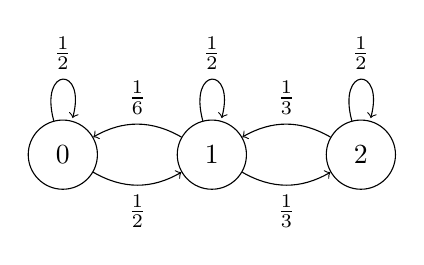
\begin{tikzpicture}
	\node[state] (0) {0};
	\node[state] (1)[right=of 0] {1};
	\node[state] (2)[right=of 1] {2};
	
	\path[->]
	(0) edge [loop above] node {$\frac{1}{2}$} (0)
	    edge [bend right] node[below] {$\frac{1}{2}$} (1)
	(1) edge [loop above] node {$\frac{1}{2}$} (1)
	    edge [bend right] node[above] {$\frac{1}{6}$} (0)
	    edge [bend right] node[below] {$\frac{1}{3}$} (2)
	(2) edge [loop above] node {$\frac{1}{2}$} (2)
	    edge [bend right] node[above] {$\frac{1}{3}$} (1);
\end{tikzpicture}
\end{center}

\theorem{Chapman-Kolmogorov Equations}
$\forall\ i,j\in S,\ n\in\nats,\ r\in[0,b]$
$$p_{ij}(n)=\sum_{k\in S}p_{ik}(r)p_{kj}(n-r)$$

\proof{Chapman-Kolmogorov Equations}
\[\begin{array}{rcll}
p_{ij}(n)&=&\prob(X_n=j|X_0=i)\\
&=&\sum_{k\in S}\prob(X_n=j|X_r=k,\ X_0=i)\prob(X_r=k|X_0=i)&\mathrm{By\ Partition\ Theorem}\\
&=&\sum_{k\in S}\prob(X_n=j|X_r=k)p_{ik}(r)&\mathrm{Markov\ Property}\\
&=&\sum_{k\in S}\prob(X_{n-r}=j|X_0=k)p_{ik}(r)&\mathrm{Time\ Homogeneity}\\
&=&\sum_{k\in S}p_{kj}(n-r)p_{ik}(r)
\end{array}\]

\proposition{Implication of Chapman-Kolmogorov Equations}
Let $P_n$ be the matrix with $(P_n)_{ij}=p_{ij}(n)$.\\
The \textit{Chapman-Kolmogorov Equations} says
$$(P_n)_{ij}=\sum_{k\in S}(P_r)_{ik}(P_{n-r})_{kj}=(P_rP_{n-r})_{ij}\\\implies P_n=P_rP_{n-r}$$
By considering $r=1$ we see that
$$P_n=PP_{n-1}=\dots=P^n$$

\subsection{Analysis by Class}

\definition{Communication}
Let $i,j\in S$. Then we can define the following relationships
\begin{enumerate}[label=\roman*)]
	\item $i$ \textit{communicates} with $j$ if $\exists\ n\geq0\ st\ p_{ij}(n)>0$. (Denoted $i\to j$).
	\item $i$ \textit{intercommunicates} with $j$ if $i\to j\ \&\ j\to i$. (Denoted $i\leftrightarrow j$).
\end{enumerate}

\proof{Intercommunication is an Equivalence Relation}
\textit{Reflexive}\\
Since $P_{ii}(0)=1$ then $i\to i\equiv i\leftrightarrow i$.\\
\textit{Symmetric}\\
let $i\leftrightarrow j$. Then
$$\implies i\to j\ \&\ j\to i\implies j\leftrightarrow i$$
\textit{Transitive}
Let $i\to j$ \& $j\to k$.\\
Then $\exists\ n,m,\in\nats\ st\ p_{ij}(n)>0\ \& p_{jk}(m).0$.\\
Thus $p_{ik}(n+m)\geq p_{ij}(n)p_{jk}(m)>0$ by \textit{Chapman-Kolmogorov Equations}.\\
$\implies i\to k$.\\
Similarly $k\to i\implies i\leftrightarrow j$.\\

\definition{Communicating Classes}
\textit{Communicating Classes} are partitions of the state set $S$ $(E_1,E_2,\dots)$ st
$$\forall\ i,j\in E_r, i\leftrightarrow j$$

\proposition{States \& Communicating Classes}
All states in the \textit{same} communicating class intercommunicate with each other.\\
Any pair of states in \textit{different} communicating classes do not intercommunicate with each other.\\

\theorem{Recurrency \& Intercommunication}
Let $i\leftrightarrow j$.\\
Then $i$ is recurrent iff $j$ is recurrent.\\

\proof{Recurrency \& Intercommunication}
Recall that state $j$ is recurrent iff $\sum_{k=0}^\infty p_{jj}(k)=\infty$.\\
Assume $j$ is recurrent \& $i\leftrightarrow j$.\\
Then $\exists\ m,n\geq0$ st $p_{ij}(m)>0\ \&\ p_{ji}(n)>0$.\\
By the \textit{Chapman-Kolmogorov} equations $p_{ii}(m+r+n)\geq p_{ij}(m)p_{jj}(r)p_{ji}(n)$.\\
Thus
$$\sum_{m,r,n}^\infty p_{ij}(m)p_{jj}(r)p_{ji}(n)=\sum_{m=0}^\infty p_{ij}(m)\sum_{r=0}^\infty p_{jj}\sum_{n=0}^\infty p_{ij}(n)>\infty$$
Thus $\sum_{n=0}^\infty p_{ii}(n)=\infty\implies$ $i$ is recurrent.\\

\remark{Recurrent \& Transient Communicating Class}
We describe a communicating class as begin\textit{recurrent} if the states in it are recurrent.\\
\nb We define \textit{Transient Communicating Classes} similarly.\\

\definition{Closed States}
A set of states $C$ is \textit{Closed} if $p_{ij}=0\ \forall\ i\in C,j\not\in C$.\\

\definition{Irreducible States}
A set of states $C$ is \textit{Irreducible} if $i\leftrightarrow j\ \forall\ i,j\in C$.\\
 
\definition{Absorbing State}
A state $i$ for which the singleton set $\{i\}$ is a closed set is called an \textit{Absorbing state}.\\
\nb $p_{ii}=1$.\\

\remark{Closed Communicating Class}
A set $E$ is closed \& irreducible iff $E$ is a closed communicating class.\\

\remark{Closed State Space}
The state space $S$ is always closed.\\

\remark{Irreducible Markov Chain}
If the state space $S$ is irreducible then we say the \textit{Markov Chain} is irreducible.\\

\example{Closed, Irreducible \& Absorbing States}
In the following state space the set of inter-communication is $\{1\leftrightarrow1,2\leftrightarrow2,3\leftrightarrow3,3\leftrightarrow4,4\leftrightarrow4\}$.\\
Hence the communicating classes are $E_1=\{1\},\ E_2=\{2\}$ \& $E_3=\{3,4\}$.\\
$E_1$ is closed \& an absorbing state.\\
$E_2$ \& $E_3$ are not closed, nor absorbing states, they are irreducible.
\begin{center}
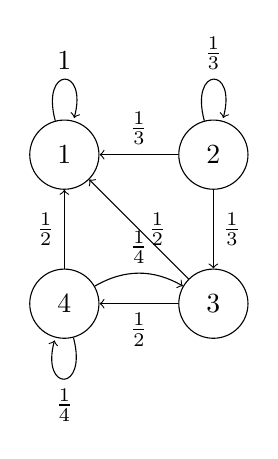
\begin{tikzpicture}
	\node[state] (1) {1};
	\node[state] (2)[right=of 1] {2};
	\node[state] (3)[below=of 2] {3};
	\node[state] (4)[below=of 1] {4};
	
	\path[->]
	(1) edge [loop above] node {$1$} (1)
	(2) edge [loop above] node {$\frac{1}{3}$} (2)
	    edge node[right] {$\frac{1}{3}$} (3)
	    edge node[above] {$\frac{1}{3}$} (1)
	(3) edge node[right] {$\frac{1}{2}$} (1)
	    edge node[below] {$\frac{1}{2}$} (4)
	(4) edge [loop below] node {$\frac{1}{4}$} (4)
	    edge [bend left] node[above] {$\frac{1}{4}$} (3)
	    edge node[left] {$\frac{1}{2}$} (1);
\end{tikzpicture}
\end{center}

\theorem{Non-Closed Communicating Classes are Transient}
If $C$ is a \textit{Communicating Class} \& $C$ is not closed, then all the states in $C$ are transient.\\

\proof{Non-Closed Communicating Classes are Transient}
Since $C$ is not closed $\exists i\in C$ \& $k\in C^c$ st $p_{ik}>0$.\\
Furthermore, since $C$ is a communicating classes and $k\not\in C$ we have $i\not\leftrightarrow k$.\\
But $i\to k$ so $k\not\to i$.
So, $f_{ki}=\prob($The chain $X$ is in state $i$ eventually$| X_0=k)=0$.\\
We compute $f_{ii}$
\[\begin{array}{rrcl}
&f_{ii}&=&\prob(X\ \mathrm{is\ in\ state\ }i\mathrm{\ eventually}|X_0=i)\\
&&=&\prob(X\ \mathrm{is\ in\ state\ }i\mathrm{\ eventually}|X_0=i,X_1=j)\prob(X_1=j|X_0=i)\\
&&=&\sum_{j\in S}\prob(X\ \mathrm{is\ in\ state\ }i\mathrm{\ eventually}|X_1=j)p_{ij}\\
&&=&\sum_{j\in S}f_{ji}p_{ij}\\
&&=&f_{ki}p_{ik}+\sum_{j\in S/\{k\}}f_{ji}p_{ij}\\
\mathrm{Since\ }f_{ki}=0&&=&\sum_{k\in S/\{k\}}f_{ji}p_{ij}\\
\mathrm{Since\ }f_{ji}\leq1&&\leq&\sum_{j\in S/\{k\}}p_{ij}\\
&&=&1-p_{ik}\\
&&=&1
\end{array}\]
Hence $i$ is transient.\\
So all states in $C$ are transient since $C$ is a communicating class.\\

\theorem{State Spaces can be Partitioned into Transient \& Recurrent States}
The state space $S$ can be uniquely partitioned into $S=T\bigcup C_1\bigcup\dots$ where $T$ is a set of transient states \& each $C_k$ is an irreducible closed set of recurrent states.\\

\proof{State Spaces can be Partitioned into Transient \& Recurrent States}
We can partition $S$ into communicating classes.\\
These classes are either recurrent or transient.\\
Let $C_k$ for $k\in\nats$ be the recurrent communicated classes \& $T$ be the union of all transient communicating classes.\\
By \textbf{Theorem 3.3} $C_k$ must be closed.\\
Thus each $C_k$ is irreducible since it is a communicating class.\\

\example{Gambler's Ruin}
Consider the following diagram for the Gambler's Ruin
\begin{center}
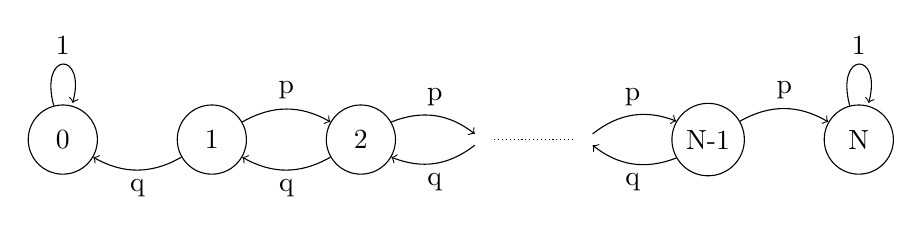
\begin{tikzpicture}
	\node[state] (0) {0};
	\node[state] (1)[right=of 0] {1};
	\node[state] (2)[right=of 1] {2};
	\node		 (m)[right=of 2] {};
	\node		 (n)[right=of m] {};
	\node[state] (3)[right=of n] {N-1};
	\node[state] (4)[right=of 3] {N};
	
	\path[->]
	(0) edge [loop above]node        {1} (0)
	(1) edge [bend left] node[below] {q} (0)
	    edge [bend left] node[above] {p} (2)
	(2) edge [bend left] node[below] {q} (1)
	    edge [bend left] node[above] {p} (m)
	(m) edge [bend left] node[below] {q} (2)
	(n) edge [bend left] node[above] {p} (3)
	(3) edge [bend left] node[below] {q} (n)
	    edge [bend left] node[above] {p} (4)
	(4) edge [loop above]node        {1} (4);
	   
   \path[draw, densely dotted]
   (m) edge (n);
\end{tikzpicture}
\end{center}
Here we have communicating classes $\{0\},\{1,\dots,N-1\}$ \& $\{N\}$.\\
$\{0\}$ \& $\{N\}$ are closed \& are absorbing states. They are recurrent.\\
$\{1,\dots,N-1\}$ is not closed since $1\to0$ \& $N-1\to N$, hence it is transient.\\

\example{Random Walk with Reflecting Barrier at 0}
Consider the following random walk which has a reflecting barrier at 0
\begin{center}
\begin{tikzpicture}
	\node[state] (0) {0};
	\node[state] (1)[right=of 0] {1};
	\node[state] (2)[right=of 1] {2};
	\node		 (m)[right=of 2] {};
	
	\path[->]
	(0) edge [loop above]node        {q} (0)
	    edge [bend left] node[above] {p} (1)
	(1) edge [bend left] node[below] {q} (0)
	    edge [bend left] node[above] {p} (2)
	(2) edge [bend left] node[below] {q} (1)
	    edge [bend left] node[above] {p} (m)
	(m) edge [bend left] node[below] {q} (2);
	   
   \path[draw, densely dotted]
   (m) edge (n);
\end{tikzpicture}
\end{center}
Here the only communicating class is $\{0,1,\dots\}$. It is closed.\\
All the states must be of the same recurrent type but which type they are depends on the values of $p$ \& $q$.\\
We shall consider computing $\prob(A|X_0=0)$ where $A=\{X$ hits $0$ eventually$\}$. There are three cases
\begin{enumerate}[label=\roman*)]
	\item $p=q=\frac{1}{2}$.\\
	\[\begin{array}{rcl}
		\prob(A|X_0=0)&=&\prob(A|X_0=0,X_1=0)\prob(X_1=0|X_0=0)+\prob(A|X_0=0,X_1=1)\prob(X_1=1|X_0=0)\\
		&=&1\times q+1\times p\\
		&=&p+q\\
		&=&1
	\end{array}\]
	Here state $0$ is recurrent.
	\item $p<q$.\\
	$$\prob(A|X_0=0)=1\times q+1\times p=1$$
	Here state $0$ is recurrent.
	\item $q>p$.\\
	$$\prob(A|X_0=0)=1\times q+\prob(A|X_1=1)p<1$$
	Here state $0$ is transient.
\end{enumerate}

\subsection{Stationary Distributions}

\definition{Stationary Distribution}
Let $\pi$ denote a \textit{horizontal vector} with a component for each state, $\pi=(\pi_1,\dots,\pi_j)$.\\
Let $X=\{X_n\}_{n\in\nats}$ be a Markov chain with transition matrix $P$.\\
We say $\pi$ is a \textit{Stationary Distribution} of the chain if
\begin{enumerate}
	\item $\pi_j\geq0\ \forall\ j\in S$ \& $\sum_{j\in S}\pi_j=1$ ($\pi$ is a mass function for $S$).
	\item $\pi=\pi P$, note that this is matrix multiplication.
\end{enumerate}
\nb Further $\pi=\pi P^n\ \forall\ n\in\nats$.\\

\example{Stationary Distribution}
Consider a Markov chain with states $S=\{0,1,2\}$ \& transition matrix $P=\begin{pmatrix}\frac{1}{2}&\frac{1}{2}&0\\\frac{1}{6}&\frac{1}{2}&\frac{1}{3}\\0&\frac{1}{2}&\frac{1}{2}\end{pmatrix}$.\\
Find a \textit{Stationary Distribution} for this chain.
\[\begin{array}{rrcl}
\mathrm{Set}&(\pi_0,\pi_1,\pi_2)&=&(\pi_0,\pi_1,\pi_2)\begin{pmatrix}\frac{1}{2}&\frac{1}{2}&0\\\frac{1}{6}&\frac{1}{2}&\frac{1}{3}\\0&\frac{1}{2}&\frac{1}{2}\end{pmatrix}\\
&&=&(\frac{\pi_0}{2}+\frac{\pi_1}{6},\frac{\pi_0}{2}+\frac{\pi_1}{2}+\frac{\pi_2}{2},\frac{\pi_1}{3}+\frac{\pi_2}{2})\\
\implies&\pi_0&=&\frac{\pi_0}{2}+\frac{\pi_1}{6}\\
\implies&\pi_0&=&\frac{\pi_1}{3}\\
\&&\pi_2&=&\frac{\pi_1}{3}+\frac{\pi_2}{2}\\
\implies&\pi_2&=&\frac{2\pi_1}{3}\\
\mathrm{Since}&\pi_0+\pi_1+\pi_2&=&1\\
\implies&\frac{\pi_1}{3}+\pi_1+\frac{2\pi_1}{3}&=&1\\
\implies&\pi_1&=&\frac{1}{2}\\
\implies&\pi&=&(\frac{1}{6},\frac{1}{2},\frac{1}{3})
\end{array}\]

\example{Random Walk with Reflecting Barrier at 0}
Consider the diagram in \textbf{Example 3.5}.\\
We are going to try and find a \textit{Stationary Distribution} for this situation.\\
\[\begin{array}{rrcll}
\mathrm{Let}&\pi&=&\pi P\\
\implies&\pi_0&=&q\pi_0+q\pi_1\\
\&&\pi_j&=&p\pi_j+q\pi_{j+1}&j\geq1\\
\implies&(1-q)\pi_0&=&q\pi_1\\
\implies&p\pi_0&=&q\pi_1\\
\&&(p+q)\pi_j&=&p\pi_{j-1}+q\pi_{j+1}&j\geq1\\
\implies&p(\pi_j-\pi_{j-1})&=&q(\pi_{j+1}-\pi_j)\\
\mathrm{Summing\ the\ first\ }j\mathrm{\ equations}&p(\pi_0-\pi_0+\pi_1-\dots-\pi_{j-1}+\pi_j)&=&q(\pi_1-\pi_1+\dots+\pi_{j+1})\\
\implies&\pi_jp&=&q\pi_{j+1}\\
\implies&\pi_{j+1}=\frac{p}{q}\pi_j\\
\implies&\pi_j&=&\left(\frac{p}{q}\right)^j\pi_0\\
\mathrm{Since}&\sum_{j=0}^\infty\pi_j&=&1\\
\implies&\sum_{j=0}^\infty\left(\frac{p}{q}\right)^j\pi_0&=&1\\
\implies&\pi_0\sum_{j=0}^\infty\left(\frac{p}{q}\right)^j&=&1\\
&&=&\begin{cases}
\infty&\mathrm{If\ }p\geq q\\
\pi_0\dfrac{1}{1-\frac{p}{q}}&\mathrm{If\ }p<q
\end{cases}
\end{array}\]
Thus $\pi$ is a stationary distribution (finite) iff $p<q$.\\

\subsection{Existence \& Uniqueness of Stationary Distributions}

\definition{Positive Recurrent}
A state $i$ is positive recurrent if the mean time of first return is finite ($m_{ii}<\infty$).\\
\nb This is a class property.\\

\theorem{Stationary Distributions in Irreducible Chains}
An \textit{Irreducible Chain} has a \textit{Stationary Distribution} $\pi$ iff all of the states are positive recurrent.\\
Here $\pi$ is unique and given by $\pi_i=\frac{1}{m_{ii}}$.\\

\theorem{}
Let $X=\{X_n\}_{n\in\nats}$ be an irreducible aperiodic \textit{Markov Chain} with a stationary distribution $\pi$. Then
$$\forall\ i,j\in S\ p_{ij}(n)\xrightarrow{n\to\infty}\pi_j$$
\nb The existence of the $\pi$ means all states are positive recurrent with $m_{ii}=\frac{1}{\pi_i}$

\subsection{Periodicity}

\definition{Period}
Let $j\in S$ be such that $p_{jj}(n)>0$ for some integers $n\geq 1$.\\
Let $\mathcal{N}_j=\{n\geq 1:p_{jj}(n)>0\}$.\\
Then the \textit{Period} of $j$ is given by $d_j=gcd(\mathcal{N}_j)$.\\

\definition{Aperiodic}
If the period of a state, $d_j$, equals $1$ then state $j$ is aperiodic.\\

\remark{}
If $p_{jj}>0$ then $J$ is aperiodic since $1\in\mathcal{N}_j$.\\

\remark{}
if $d_j\geq2$ then $p_{jj}(n)$ cannot possibly converge, except occasionally to 0.\\

\theorem{Period within a Communicating Class}
Let $C\subseteq S$ be a communicating class of states.\\
Let $i,j\in C$.\\
Then $d_i=d_j$.\\

\proof{Period within a Communicating Class}
Suppose $d_i\neq d_j$, and without loss of generality assume $d_i<d_j$.\\
Since $C$ is a communicating class, $i\leftrightarrow j$, and there exists $m\geq0,\ n\geq0$ st $p_{ij}(m)>0$ and $p_{ji}(n)>0$.\\
Suppose $p_{ii}(s)>0$.\\
Then $p_{ii}(rs)\geq r.p_{ii}(s)>0$ for $r\in\nats$.\\
Therefore $p_{jj}(n+rs+m)\geq p_{ji}(n)p_{ii}(rs)p_{ij}(m)>0$ so $(n+rs+m)\in\mathcal{N}_j$.\\
In particular, both $(n+s+m)$ and $(n+2s+m)$ are multiples of $d_j$, so $s=(n+2s+m)-(n+s+m)=s$ is a multiple of $d_j$.\\
We have shown that $d_j$ is a divisor of all the values of $s$ such that $p_{ii}(s)>0$.\\
$d_i$ is defined to be the $gcd$ of the same set of $s$ values, so $d_i\geq d_j$.\\
But we started by assuming $d_i<d_j$.\\
This is a contradiction.\\
So we must have $d_i=d_j$.\\

\example{Period}
Let $S=\{0,1\}$ and with transition matrix $P=\begin{pmatrix}0&1\\1&0\end{pmatrix}$.\\
So $p_{00}(n)=\begin{cases}0&\mathrm{if\ }n\mathrm{\ is\ odd}\\1&\mathrm{if\ }n\mathrm{\ is\ even}\end{cases}$.\\
Since $p_{00}(n)>0$ only when $n$ is event, the period must be a multiple of 2.\\
And, since $p_{00}(2)>0$, the period must be no more than 2.\\
Therefore $d_0=2$.\\

\section{Markov Chains in Continuous Time}

\definition{Lack of Memory Property}
Let $X$ be a random variable.\\
$X$ is said to have the \textit{Lack of Memory Property} if
$$\prob(X>t+h|T>h)=\prob(T>h)$$

\remark{Distributions with Lack of Memory Property}
The \textit{Exponential Distribution} has the \textit{Lack of Memory Property}.\\

\proposition{Modelling Wait Times}
LET $T$ be a random variable that models wait times between events.\\
Then $T$ should have the following property
\[\begin{array}{rrcl}
&\prob(T\in(t,t+h]|T>t)&=&\lambda h+o(h)\\
\implies&\prob(T>t+h|T>t)&=&1-\lambda h+o(h)
\end{array}\]
\nb $\lim\limits_{h\to0}\frac{0(h)}{h}=0$.\\

\proposition{Distribution for Modelling Wait Times}
Consider the $T$ defined in \textbf{Proposition 4.1}.\\
Let $g(t)=\prob(T>t)$. Then
\[\begin{array}{rrcl}
&g(t+h)&=&\prob(T>t+h)\\
&&=&\prob(T>t+h|T>t)\prob(T>t)+\prob(T>t+h|T\leq t)\prob(T\leq t)\\
&&=&(1-\lambda h+o(h))g(t)+0\\
&&=&(1-\lambda h)g(t)+o(h)\\
\implies&\dfrac{g(t+h)-g(t)}{h}&=&\dfrac{-\lambda hg(t)}{h}=\dfrac{o(h)}{h}\\
\implies g'(t)&=&-\lambda g(t)+0\\
\implies g(t)&=&-\frac{g'(t)}{\lambda}\\
&=&ce^{-\lambda t}
\end{array}\]
Since $g(0)=1\implies1=ce^0\implies c=1\implies g(t)=e^{-lambda t}$.\\
So $T\sim Exp(\lambda)$.\\

\example{Who arrives first?}
Consider having arranged to meet with $n$ friends.\\
Let $T_i$ be the length of time you wait for the $i^{th}$ first to arrived.\\
Assume the $T_i$s are independent and identically distributed with $T_i\sim Exp(\lambda_i)$.\\
\begin{enumerate}[label=\roman*)]
	\item Derive the distribution of the length of time until the first friend turns up.
	\[\begin{array}{rrcl}
		&\prob(min(T_1,...,T_n)>t)&=&\prob(t_1>t,\dots,T_n>T)\\
		&&=&\prod_i\prob(T_i>t)\mathrm{\ by\ indepdence}\\
		&&=&\prod_ie^{-\lambda_it}\\
		&&=&e^{-t\sum_i\lambda_i}\\
		\implies&min(T_1,\dots,T_n)&\sim&Exp\left(\sum_{i=1}^n\lambda_i\right)
	\end{array}\]
	\item Derive the probability that the first friend to turn up is friend i.\\
	\[\begin{array}{rcl}
	\prob(i^{th}\ friend\ is\ first)&=&\prob(T_i=min(T_1,\dots,T_n))\\
	&=&\prob(T_i<T_j,j\neq i)\\
	&=&\int\limits_0^\infty\prob(T_j>T_i,j\neq i|T_i=t)dt\\
	&=&\int\limits_0^\infty\prob(T_j>t,j\neq i)\lambda e^{-\lambda_it}dt\\
	&=&\int\limits_0^\infty\prod\limits_{j=1,j\neq i}^n\prob(T_j>t)\lambda_ie^{-\lambda_i}dt\mathrm{\ by\ independce}\\
	&=&\int\limits_0^\infty e^{-t\sum_{j\neq i}\lambda_j}\lambda_ie^{-\lambda_it}dt\\
	&=&\lambda_i\int\limits_0^\infty e^{-t\sum_{i=1}^n\lambda_i}dt\\
	&=&\lambda_i\left[\dfrac{exp\left(-t\sum_{i=1}^n\lambda_i\right)}{-\lambda_{i=1}^n\lambda_i}\right]_0^\infty\\
	&=&\dfrac{\lambda_i}{\sum_{i=1}^n\lambda_i}
	\end{array}\]
\end{enumerate}

\proposition{Link Exponential \& Binomial Distribution}
Consider the time till occurrence of an event is modelled by $Exp(\mu)$.\\
So the probability of the event occurring before time $t$ is $1-e^{-\mu t}\approx\mu t$ if $\mu t$ is small.\\
If there are $n$ independent events with the same distribution we can model the number of events that occur by time $t$ with $Bi(n,\mu t)$

\subsection{Poisson Process}

\definition{Poisson Process}
Let $\{N_t\}_{t\geq0}$ be a continuous time stochastic process where $N_t$ counts the number of events to have occurred by time $t$.\\
$\{N_t\}_{t\geq0}$ is a \textit{Poisson Process} with rate $\lambda$ if
\begin{enumerate}[label=\roman*)]
	\item $N_t\in\nats\ \forall\ t\geq0$;
	\item $N_0=0$;
	\item It has stationary increments \textit{i.e.} $N_{t+s}-N_t$ depends only on $s$;
	\item It has independent increments \textit{i.e.} $N_{t_2}-N_{t_1},\dots,N_{t_n}-N_{t_{n-1}}$ are independent;
	\item If $t>0$ and $h>0$ then
	\[\begin{array}{rcl}
	\prob(N_{t+h}-N_t<0)&=&0\\
	\prob(N_{t+h}-N_t=0)&=&1-\lambda h+o(h)\\
	\prob(N_{t+h}-N_t=1)&=&\lambda h+o(h)\\
	\prob(N_{t+h}-N_t>1)&=&o(h)
	\end{array}\]
	as $h\to0$.
\end{enumerate}
\nb $\lim\limits_{h\to0}\frac{o(h)}{h}=0$.\\

\theorem{Distribution of Poisson Process}
for $t\geq0$
$$N_t\sim Po(\lambda t)$$

\proof{Theorem 4.1}
%TODO

\proposition{Implications of Theorem 4.1}
From \textbf{Theorem 4.1} it follows that $\expect(N_t)=Var(N_t)=\lambda t$.\\
Since $N_0=0$ we have stationary increments
$$N_{t+s}-N_t\sim N_s-N_0=N_S-0\sim N_S\sim Po(\lambda s)$$
Thus the number of events in any interval of width $s$ is distributed by $Po(\lambda s)$.\\

\proposition{Distribution of Initial Arrival Time}
Let $S_1$ be the time of the first arrival, so $S_1=inf\{t\geq0:N_t>0\}$.\\
Consider the event $\{S_1>t\}$.\\
We have that $\{S_1>t\}\equiv\{N_t=0\}$.\\
Hence $\prob(S_1>t)=\prob(N_t=0)=e^{-\lambda t}$ since $N_t\sim Po(\lambda t)$.\\
Thus $S_1\sim Exp(\lambda)$.\\

\proposition{Distribution of General Arrival Time}
Let $S_n$ be the time of the $n^{th}$ arrival, so $S_n=inf\{t\geq0:N_t=n\}$.\\
Consider the event $\{S_n>t\}$.\\
We have that $\{S_n>t\}\equiv\{N_t<n\}$.\\
Let $T_i$ be the inter-arrival times st $T_1=S_1,\ T_2=S_2-S_1,\dots,T_n=S_n-S_{n-1}$.\\
Note that $S_n=\prod_{i=1}^nT_i$.
\[\begin{array}{rcll}
\prob(T_n>t|S_{n-1}=s_{n-1},\dots,S_1=s_1)&=&\prob(N_{t+s_{n-1}}-N_{s_{n-1}}=0|S_{n-1}=s_{n-1},\dots,S_1=s_1)\\
&=&\prob(N_{t+s_{n-1}}-N_{s_{n-1}}=0)\mathrm{\ by\ indepdent\ increments}\\
&=&\prob(N_t-N_0=0)\mathrm{\ by\ stationary\ increments}\\
&=&\prob(N_t=0)\\
&=&e^{-\lambda t}
\end{array}\]
Since $e^{-\lambda t}$ is independent of $s_1,\dots,s_{n-1}\implies T_n$ is independent of $S_1,\dots,S_{n-1}$.\\
Hence $T_n$ is independent of $T_1,\dots,T_{n-1}$ be definition.\\
So $T_i\sim Exp(\lambda)\ \forall\ i$.\\
Hence $S_n=\sum_{i=1}^nT_i\sim\Gamma(n,\lambda)$.

\subsection{Birth Death Process}

\subsubsection{Linear Birth Processes}

\definition{Linear Birth Process}
Consider a population of individuals.\\
In the \textit{Linear Birth Process} each individual present at time $t$ splits into 2 during the interval $(t,t+h)$ with probability $\lambda h+o(h)$.\\
We have that all individuals act independently of each other.\\
\nb The birth rate is independent of the population size.\\
\nb This is also known as a \textit{Yule Process}.\\
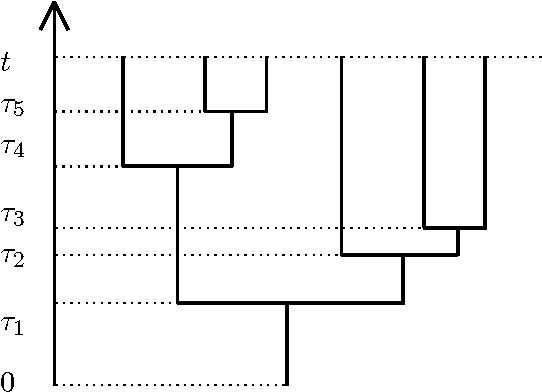
\includegraphics[scale=0.2]{img/yule.png}\\

\proposition{Distribution of Time between Arrivals}
Let $N_t$ be the population size at time $t$, assume $N_0=1$.\\
For $n\geq 1$ let $S_n$ be the time until the population reaches size $n$, so $S_n=inf\{t\geq0:N_t=n\}$.\\
Let $T_j$ be the time to grow from size $j$ to $j+1$, so $T_j=S_{j+1}-S_j$.\\
Consider a population of size $j$.\\
Let $Y_i$ be hte waiting time until $i^{th}$ individual splits.\\
then, by definition \& \textbf{Proposition 4.2}, we have that $Y_1,\dots,Y_j$ are iid with distribution $Exp(\lambda)$.\\
We have that $T_j=min\{Y_1,\dots,Y_j\}$.\\
Since $T_j\sim Exp(k\lambda)\implies\expect(T_j)=\frac{1}{j\lambda}$.\\
Using $S_n=T_1+\dots+T_{n-1}$ we have that
$$\expect(S_n)=\expect(T_1+\dots+T_{n-1})=\frac{1}{\lambda}(1+\frac{1}{2}+\dots+\frac{1}{n-1})$$
This is not convergent but can be approximated to $\frac{1}{\lambda}\int_1^n\frac{1}{x}dx=\frac{1}{\lambda}\log_n$.\\

\proposition{Distribution of Number of Births}
For a population of size $n$ each has an independent probability of $\lambda h+o(h)$ for giving birth in interval $(t,t+h)$.\\
The distribution of number of births in time period $(t,t+h)$ is
$$Bi(n,\lambda h+o(h))$$

\proposition{Distribution of Population Size, $N_t$}
Let $N_t$ denote the size of the population at time $t$ with birth rate $\lambda$, then
$$N_T\sim Geo(e^{-\lambda t})$$
\nb $\expect(N_t)=e^{\lambda t}$.

\subsubsection{Linear Birth \& Death Processes}

\definition{Linear Birth \& Death Process}
Consider an individual in a population \& the possible events that can occur to them in $(t,t+h)$.\\
In a \textit{Linear Birth \& Death Process} these are
\begin{enumerate}[label=\roman*)]
	\item Gives birth, splits in two, with probability $\lambda h+o(h)$;
	\item Dies with probability $\mu h+o(h)$; or,
	\item Neither event, with probability $1-(\lambda+\mu)h+o(h)$.
\end{enumerate}
\nb We can consider the random variables $B\sim Exp(\lambda)$ \& $D\sim Exp(\mu)$.\\
\nb The birth \& death rates are independent of the population size.\\

\proposition{Probability of Birth or Death}
Given an event has occurred:
\begin{enumerate}[label=\roman*)]
	\item The probability it was a birth is $\dfrac{\lambda}{\lambda+\mu}$
	\item The probability it was a death is $\dfrac{\mu}{\lambda+\mu}$
\end{enumerate}

\subsubsection{Generalised Birth \& Death Processes}

\definition{Generalised Birth \& Death Process}
A continuous time stochastic process $\{N_t\}_{t\geq 0}$ is a \textit{Generalised Birth \& Death Process} if
\begin{itemize}
	\item[-] $N_t\in\nats_0$;
	\item[-] $\prob(N_{t+h}-N_t=1|N_t=n)=\lambda_nh+o(h)$
	\item[-] $\prob(N_{t+h}-N_t=-1|N_t=n)=\mu_nh+o(h)$
	\item[-] $\prob(N_{t+h}-N_t=0|N_t=n)=1-(\lambda_n+\mu_n)h+o(h)$
	\item[-] $\lambda_n,\mu_n\geq0\ \forall\ n$;
	\item[-] $\mu_0=0$.
\end{itemize}
\nb The birth and death rate depends upon the size of the population.\\

\proposition{General Rate of Change}
Let $p_n(t)=\prob(N_t=n)$.\\
Then
$$p'_n(t)=\lambda_{n-1}p_{n-1}(t)-(\lambda_n+\mu_n)p_n(t)+\mu_{n=1}p_{n+1}(t)\ \forall\ n\geq 1$$
and
$$p_0'(t)=-\lambda_0p_0*t)+\mu_1p_1(t)$$

\example{Stationary Distribution - Constant Birth Rate \& Increasing Death Rate}
Consider a situation where $\lambda_n=\lambda>0\ \forall\ n\in\nats$ \& $\mu_n=\mu n\forall\ n\in\nats$.\\
Derive the stationary distribution for this process
\
Let $p_n(t)=\prob(N_t=n)$. From the general formula in \textbf{Proposition 4.11} we have
$$p_n'(t)=\lambda p_{n-1}(t)-(\lambda+\mu n)p_n(t)+\mu(n+1)p_{n+1}(t)$$
Consider the case that $n=0$
\[\begin{array}{rrcl}
&p_0(t+h)&=&\prob(N_{t+h}=0)\\
&&=&\prob(N_{t+h}=0|N_t=0)\prob(N_t=0)+\prob(N_{t+h}=0|N_t=1)\prob(N_t=1)+o(h)\\
&&=&(1-\lambda h)p_0(t)+\mu hp_1(t)+o(h)\\
\implies&\dfrac{p_0(t+h)-p_0(t)}{h}&=&-\lambda p_0(t)+\mu p_1(t)
\end{array}\]
Let $h\to0\implies p_0'(t)=-\lambda p_0(t)+\mu p_1(t)$.\\
We assume the process reaches a steady space where it no longer changes, this occurs at large $t$.\\
Then means $\exists \hat{p}_n$ where
$$p_n(t)\xrightarrow{t\to\infty}\hat{p}_n\ \&\ \hat{p}_n'(t)\to 0$$
By the general formula \& derivative of $\hat{p}_0$ we have that
\[\begin{array}{rcl}
0&=&\lambda\hat{p}_{n-1}-(\lambda+\mu n)p_n+\mu(n+1)\hat{p}_{n+1}\\
0&=&-\lambda\hat{p}_0+\mu\hat{p}_1
\end{array}\]
Rearranging gives
\[\begin{array}{rcl}
\mu(n+1)\hat{p}_{n+1}-\lambda\hat{p}_{n}&=&\mu_n\hat{p}_{n}-\lambda\hat{p}_{n+2}\\
&\dots&\\
&=&\mu\hat{p}_{1}-\lambda\hat{p}_{0}=0
\end{array}\]
Hence $\mu n\hat{p}_{n}-\lambda\hat{p}_{n-1}=0\ \forall\ n\in\nats$.\\
$$\implies\hat{p}_{n}=\dfrac{\lambda}{\mu n}\hat{p}_{n-1}=\dots=\dfrac{1}{n!}\left(\frac{\lambda}{\mu}\right)^n\hat{p}_{0}$$
Normalising
\[\begin{array}{rcl}
1&=&\sum_{n=0}^\infty\hat{p}_{n}\\
&=&\sum_{n=0}^\infty\frac{1}{n!}\left(\frac{\lambda}{\mu}\right)\hat{p}_{0}\\
&=&\hat{p}_{0}e^{\lambda/\mu}\\
\implies\hat{p}_{0}&=&e^{-\lambda/\mu}
\end{array}\]
Thus $\hat{p}_{n}=\frac{1}{n!}\left(\frac{\lambda}{\mu}\right)e^{-\lambda/\mu}\ \forall\ n\in\nats^0$.\\
This stationary distribution is distributed $\sim Po\left(\frac{\lambda}{\mu}\right)$.\\

\subsection{General Markov Chains in Continuous Time}

\definition{Generator}
$G$ is the \textit{Generator} of a \textit{Markov Chain} where $G$ satisfies
\begin{enumerate}[label=\roman*)]
	\item $g_{ij}\geq0$ for $j\neq i$;
	\item $g_{ii}\leq0$; and
	\item $\sum_{j\in S}=0$.
\end{enumerate}
\nb $g_{ii}=-\sum_{j\neq i}g_{ij}$.\\

\proposition{Chains \& Their Generator}
For reasonable chains it can be shown that
\[\begin{array}{rcl}
p_{ij}(h)&=&g_{ij}h+o(h)\ \mathrm{for\ }i\neq j\\
p_{ii}(h)&=&1-\sum_{j\neq i}p_{ij}(h)\\
&=&1-\sum_{j\neq i}g_{ij}h+o(h)\\
&=&1+g_{ii}h+o(h)
\end{array}\]

\example{Linear Birth \& Death Process}
We know that
$$\prob(N_{t+h}=j|N_t=i)=p_{ij}(h)=\begin{cases}\mu ih+o(h)&\mathrm{if\ }j=i-1\\\lambda ih+o(h)&\mathrm{if\ }j=i+1\\1-(\lambda+\mu)hi+o(h)&\mathrm{if\ }j=i\\o(h)&\mathrm{otherwise}\end{cases}$$
Using $p_{ij}(h)=g_{ij}h+o(h)$ \& $p_{ii}(h)=g_{ii}h+1+o(h)$
$$g_{ij}=\begin{cases}\mu&\mathrm{j=i-1}\\\lambda&\mathrm{j=i+1}\\-(\lambda+\mu)i&\mathrm{j=i}\\0&\mathrm{otherwise}\end{cases}$$

\definition{Forward Equations}
The \textit{Forward Equations} is given as
$$(P_t')_{ij}=(P_tG)_{ij}$$
Since this holds $\forall\ i,j$ we have $P_t'=P_tG$ \& $P_0=I$.\\

\proposition{Deriving Forward Equations}
Consider the probability of being in state $j$ at time $t+h$ if the chain started in $i$ at time $0$, $p_{ij}(t+h)$.\\
Conditioning on the state of the chain at time $t$ we get
\[\begin{array}{rcl}
p_{ij}(t+h)&=&\prob(X_{t+h}=j|X_0=i)\\
&=&\sum_{k\in S}\prob(X_{t+h}=j|X_t=k,X_0=i)\prob(X_t=k|X_0=i)\\
&=&\sum_{k\in S}\prob(X_t=k,X_0=i)\prob(X_t=k|X_0=i)\mathrm{\ by\ Markov\ Property}\\
&=&\sum_{k\in S}p_{kj}(h)p_{ik}(t)\\
&=&p_{jj}(h)p_{ij}(t)+\sum_{k\in S/\{s\}}p_{kj}(h)p_{ik}(t)\\
&=&(1+g_{jj}h+o(h))p_{ij}(t)+\sum_{k\in S/\{j\}}(g_{kj}h+o(h))p_{ik}(t)\\
&=&p_{ij}(t)+\sum_{k\in S}g_{kj}hp_{ik}(t)+o(h)\\
\implies\dfrac{p_{ij}(t+h)-p_{ij}(t)}{h}&=&\sum_{k\in S}g_{kj}p_{ik}(t)+\dfrac{o(h)}{h}\\
\implies p_{ij}'(t)&=&\sum_{k\in S}g_{kj}p_{ik}(t)\\
\implies (P_t')_{ij}&=&(P_tG)_{ij}
\end{array}\]

\proposition{Solving Forward Equations}
We can solve the \textit{Forward Equations} as ordinary differential equations
\[\begin{array}{rrcl}
&P_t'-P_tG&=&0\\
\implies&I(t)&=&e^{-\int Gdt}=e^{-Gt}\\
\implies&\frac{d}{dt}(e^{-Gt}P_t)&=&0\\
\implies&e^{-G}P_t&=&C\mathrm{\ some\ matrix}\\
\implies&e_0P_0&=&C\\
\implies&1I&=&C\\
\implies&C&=&I\\
\implies&P_t&=&e^{Gt}
\end{array}\]

\theorem{}
$$\frac{d^k}{dt^k}\bigg|_{t=0}P_t=G_k\ \forall\ k\geq 0$$

\proof{Theorem 4.2}
\[\begin{array}{rcl}
\frac{d^k}{dt^k}\bigg|_{t=0}P_t&=&\frac{d^k}{dt^k}\bigg|_{t=0}\sum\limits_{n=0}^\infty\dfrac{t^n}{n!}G^n\\
&=&\sum\limits_{n=0}^\infty\frac{d^k}{dt^k}\bigg|_{t=0}\dfrac{t^n}{n!}G^n\\
&=&\sum\limits_{n=0}^\infty\frac{t^{n-k}}{(n-k)!}\bigg|_{t=0}G^n\\
&=&G^k
\end{array}\]

\example{Computing $P_t$ from $G$}
Consider the state space $S=\{1,2,3\}$ with $G=\begin{pmatrix}-2&1&1\\1&-1&0\\2&1&-3\end{pmatrix}$.\\
We partially diagonalise $G$.\\
Setting $|G-\lambda I|=0$ we get $\lambda_1=0,\lambda_2=-2\ \&\ \lambda_3=-4$.\\
Since the eigenvalues are distinct $\exists U\in M_3$ st
\[\begin{array}{rcl}
G&=&U\begin{pmatrix}0&0&0&\\0&-2&0\\0&0&-4\end{pmatrix}U^{-1}\\
\implies G^n&=&U\begin{pmatrix}0^n&0&0&\\0&(-2)^n&0\\0&0&(-4)^n\end{pmatrix}U^{-1}
\end{array}\]
We know that $P_t=e^{tG}$ so
\[\begin{array}{rcl}
P_t&=&\sum\limits_{n=0}^\infty\dfrac{t^nG^n}{n!}\\
&=&\sum\limits_{n=0}^\infty\dfrac{t^n}{n!}U\begin{pmatrix}0^t&0&0&\\0&(-2)^t&0\\0&0&(-4)^t\end{pmatrix}U^{-1}\\
&=&U\begin{pmatrix}\sum_{n=0}^\infty\frac{0^n}{n!}&0&0&\\0&\sum_{n=0}^\infty\frac{(-2t)^n}{n!}&0\\0&0&\sum_{n=0}^\infty\frac{(-4t)^n}{n!}\end{pmatrix}U^{-1}\\
&=&U\begin{pmatrix}e^0&0&0&\\0&e^{-2t}&0\\0&0&e^{-4t}\end{pmatrix}U^{-1}\\
\end{array}\]
Hence $P_{ij}(t)=a_{ij}+b_{ij}e^{-2t}+c_{ij}e^{-4t}\ \forall\ i,j\in S$.
Using \textbf{Theorem 4.2} \& considering $i=j=1$ we have
\[\begin{array}{rcl}
P_{11}(t)&=&a_{11}+b_{11}e^{-2t}+c_{11}e^{-4t},\\
P_{11}'(t)&=&-2b_{11}e^{-2t}-4c_{11}e^{-4t}\\
\&\ P_{11}''(t)&=&4b_{11}e^{-2t}+16c_{11}e^{-4t},\\
\end{array}\]
Setting $t=0$
\[\begin{array}{rcl}
P_{11}(0)&=&(G^0)_{11}\\
&=&a_{11}+b_{11}+c_{11}\\
P_{11}'(0)&=&(G^1)_{11}=-2\\
&=&-2b_{11}-4c_{11}\\
P_{11}''(0)&=&(G^2)_{11}\\
&=&(-2)^2+(1\times1)+(2\times 1)=7\\
&=&4b_{11}+16c_{11}
\end{array}\]
Solving this series of simultaneous equations we get
$$a_{11}=\frac{3}{8},\ b_{11}=\frac{1}{4}\ \&\ c_{11}=\frac{3}{8}$$ 

\example{Exponential Holding Times}
Assume at time $t$ the chain enters state $i$ \& then stays in $i$ for some random time $U=inf\{s\geq0:X_{t+s}\neq i\}$. It the jumps to a new state.\\
Let $h_{ij}$ be the probability it jumps from state $i$ to state $j$, with $h_{ii}=0$.\\
We have that
\[\begin{array}{rcl}
\prob(U>u+v|U>v)&=&\prob(U>v+u|X_{t+u}=i\mathrm{\ and\ further\ information\ about\ the\ past})\\
&=&\prob(U>v) \mathrm{by\ Markov\ property}
\end{array}\]
Since $U$ has last of memory property \& is on continuous time it must have an exponential distribution.\\
Let $U\sim Exp(\lambda_i)$. We shall relate the values of $\lambda_i$ \& $h_{ij}$ to the generator matrix $G$.\\
For $i\neq j$. Since $g_{ij}=p_{ijj}'(0)$ then
\[\begin{array}{rcl}
g_{ij}&=&\lim_{\delta\to0}\frac{p_{ij}(delta)-p_{ij}(0)}{\delta}\\
&=&\lim_{\delta\to0}\frac{p_{ij}(delta)-0(0)}{\delta}\\
&=&\lim_{\delta\to0}\frac{\prob(\mathrm{in\ time} (0,\delta),\mathrm{leave\ state\ }i,\mathrm{jump\ to\ }j,\ \mathrm{and\ nothing\ else)}+o(\delta)}{\delta}\\
&=&\lim_{\delta\to0}\frac{\prob(U<\delta)h_{ij}+o(\delta)}{\delta}\\
&=&\lim_{\delta\to0}\frac{(1-e^{-\lambda_i\delta})h_{ij}+o(\delta)}{\delta}\\
&=&\lambda_ih_{ij}\mathrm{\ by\ l'H\hat{o}pital's\ rule}
\end{array}\]
For $i=j$
\[\begin{array}{rcl}
g_{ii}&=&\lim_{\delta\to0}\frac{p_{ii}(delta)-p_{ii}(0)}{\delta}\\
&=&\lim_{\delta\to0}\frac{e^{-\lambda_i\delta}+o(\delta)-1}{\delta}\\
=-\lambda_i\mathrm{\ by\ l'H\hat{o}pital's\ rule}
\end{array}\]
Rearranging this we see that
\[\begin{array}{rrcl}
&\lambda_i&=&-g_{ii}\\
&h_{ij}&=&\dfrac{g_{ij}}{\lambda_i}\\
&&=&-\dfrac{g_{ij}}{g_{ii}}>0\\
\implies&\sum_{j\in S}h_{ij}&=&\sum_{j\neq i}-\frac{g_{ij}}{g_{ii}}+h_{ii}\\
&&=&\sum_{j\neq i}-\frac{g_{ij}}{g_{ii}}\\
&&=&1
\end{array}\]
Thus the matrix $H$ is a stochastic matrix.\\
The chain $X_t$ proceeds with a sequence of jumps around the state space.\\

\definition{Jump Chain}
Let $S_1<S_2<\dots$ denote the times when the continuous-time Markov Chain $X$ jumps.\\
The discrete-time Markov Chain formed by $(X_{S_1},X_{S_2},\dots)$ is called the \textit{Jump Chain}.\\
\nb This is AKA \textit{Embedded Markov Chain}.\\

\example{Jump Chain for Linear Births \& Deaths}
Define
$$p_{ij}(h)=\begin{cases}o(h)&j<i-1\ or\ j>i+1\\\mu ih+o(h)&j=i-1\\1-(\lambda+\mu)ij+o(h)&j=i\\\lambda ih+o(h)&j=i+1\end{cases}$$
and
$$g_{ij}=\begin{cases}0&j<i-1\ or\ j>i+1\\\mu i&j=i-1\\-(\lambda+\mu)i&j=i\\\lambda i&j=i+1\end{cases}$$
Note that $U\sim Exp(-g_{ii})\sim Exp((\lambda+\mu)i)$.\\
Hence, the jump chain transition probabilities are
$$h_{ij}=\begin{cases}0&j<i-1\ or\ j>i+1\\\frac{\mu}{\lambda+\mu}&j=i-1\\\frac{\lambda}{\lambda+\mu}&j=i+1\\0&j=i\end{cases}$$

\subsection{Class Structure, Recurrence \& Stationary Distributions}

\definition{Equivalent Definitions of Communication}
If $i\neq j$ the following are equivalent
\begin{enumerate}[label=\roman*)]
	\item $i\to j$;
	\item $i\to j$ in the jump chain;
	\item $\exists i\neq i_1\neq\dots\neq i_n\neq j$ st $g_{ii_1}g_{i_1i_2}\dot g_{i_nj}>0$;
	\item $p_{ij}(t)>0\ \forall\ t$
\end{enumerate}

\definition{Continuous Time Recurrence}
A state $i$ is called \textit{Recurrent} in continuous time if $\prob(\{t\geq0:X_t=i\}\ is\ unbounded|X_0=i)=1$.\\

\definition{Continuous Time Transience}
A state $i$ is called \textit{Transient} in continuous time if $\prob(\{t\geq0:X_t=i\}\ is\ unbounded|X_0=i)=0$.\\

\theorem{}
A state $i$ is recurrent for the continuous time Markov Chain $X_t$ iff it is recurrent for the jump chain $Y_n$.\\

\proof{Theorem 4.3}
Suppose $X_0=Y_0=i$ and let $_n$ be the $n^{th}$ jump time of $X_t$.\\
Suppose $i$ is recurrent for $Y_n$ so that $Y_n=i$ for infinitely many $n$ with probability $1$.\\
Hence $X_{T_n}=Y_n=i$ for infinitely many $n$, and the set $\{t:X_t=i\}$ is unbounded with probability $1$.\\
So $i$ is recurrent for $X_t$.\\
\\
Conversely, suppose that $i$ is transient for $Y_n$.\\
So $\prob(Y_n=i\ infinitely\ often)=0$ and with probability 1 there xists a maximal $n$ st $Y_n=i$.\\
Therefore $X_t\neq i\ \forall\ t>T_{n+1}$.\\
Thus $i$ is transient for $X_t$.\\

\theorem{Stationary Distribution \& Generator}
If $P_t$ has generator $G$ then $\pi$ is stationary iff $\pi G=0$.\\

\proof{Theorem 4.4}
We have
\[\begin{array}{rcl}
\pi\mathrm{\ is\ stationary}&\Leftrightarrow&\pi P_t=\pi\ forall\ t\geq0\\
&\Leftrightarrow&\frac{d}{dt}\pi P_t=\frac{d}{dt}\pi\\
&\Leftrightarrow&\pi P_t'=0\\
&\Leftrightarrow&\pi GP_t=0\mathrm{\ by\ backwards\ equations}
\end{array}\]
But for $t=0,\ P_0=I\implies \pi GP_0=\pi G=0$.\\

\theorem{}
Let $G$ be the generator of a chain whose jump chain has transition matrix $H$.\\
Then $\pi$ is stationary for $G$ iff $vH=v$ where $([v]_i=\pi_ig_{ii}$.\\

\proof{Theorem 4.5}
\[\begin{array}{rrcl}
&vH&=&v\\
\implies&vH-vI&=&0\\
&[v(H-I)]_j&=&\sum_{i\in S}v_i(h_{ij}-\delta{ij})\\
&&=&v_j(h_{jj}-\delta_{jj}\sum_{i\neq j}v_i(h_{ij}-0)\\
&&=&(-\pi_jg_{jj})(-1)+\sum_{i\neq j}-\pi_ig_{ii}\left(\frac{-g_{ij}}{g_{ii}}\right)\\
&&=&\sum_{i\in S}\pi_ig_{ij}\\
&&=&[\pi  G]_g\\
\implies&(\pi G)=0&\Leftrightarrow&vH=v\\
&&\Leftrightarrow&\pi\mathrm{\ stationary}
\end{array}\]

\theorem{}
For an irreducible continuous time Markov chain
$$p_{ij}\xrightarrow{t\to\infty}\pi_j$$

\section{Brownian Motion}

\subsection{Basic Notions}

\remark{Brownian Motion Intuition}
\textit{Brownian Motion} can be though of as the motion of a particle suspended in fluid, moving randomly but continuously about $\real^n$ with $n\in\nats$.\\

\definition{Multivariate Normal Distribution}
An $n\times1$ random vector $\pmb{X}=(X_1,\dots,X_n)^t$ has \textit{Multivariate Normal Distribution} if its joint density is
$$f(\pmb{x})=\frac{1}{(2\pi)^{n/2}|\Sigma|^{1/2}}exp\left(-\frac{1}{2}(\pmb{x}-\pmb{\mu})^t\Sigma^{-1}(\pmb{x}-\pmb{\mu})\right)$$
where $\Sigma$ is a symmetric positive-definite matrix of size $n\times n$ and $\pmb{\mu}$ is a $n\times 1$ vector.\\
\nb - This distribution is denoted $N(\pmb{\mu},\Sigma)$.\\
\nb - This is also known as \textit{Multinormal Distribution}.\\

\remark{Positive-Definite Matrix}
Let $A$ be a symmetric positive-definite matrix of size $n\times n$.\\
Then $A$ has $n$ eigenvalues which are all positive.\\
Furthermore, we can define $A=P^{-1}DP$ where $D$ is a diagonal matrix of the eigenvalues \& $P$ is a unitary matrix.\\

\theorem{Properties of Multivariate Normal Distribution}
If $\pmb{X}\sim N(\pmb{\mu},\Sigma)$ then
\begin{enumerate}[label=\roman*)]
	\item $\expect(\pmb{X})=\mu$ (\textit{i.e.} $\expect(X_i)=\mu_i$;
	\item The $i,j^{th}$ entry of $\Sigma$ is the $Cov(X_i,X_j)$.\\
\end{enumerate}

\theorem{Distribution of Linear Transformation of Multinormal Distribution}
Let $m\leq n$.\\
Define $\pmb{X}\sim N(\pmb{\mu},\Sigma)$ to be a $n\times 1$ random vector, $\pmb{c}\in\real^{m}$ \& $B\in\real^{m\times n}$ with $Rank(B)=m$. Then
$$\pmb{Y}=\pmb{c}+B\pmb{X}\implies\pmb{Y}\sim N(\pmb{c}+B\pmb{\mu},B\Sigma B^t)$$

\remark{MultiNormal Distribution of Independent Variables}
Let $\pmb{X}=(X_1,\dots,X_n)^t$ with $X_1,\dots,X_n$ be independent with distributions $X_i\sim N(\mu_i,\sigma_i^2)$.\\
Then $\pmb{X}\sim N(\pmb{\mu},Diag_n(\sigma^2_i))$ where $\pmb{\mu}=(\mu_1,\dots,\mu_n)^t$ and $Diag_n(\sigma_i^2)=\begin{pmatrix}\sigma_1^2&0&\dots&0\\0&\sigma_2^2&\dots&0\\\vdots&\vdots&\ddots&\vdots\\0&0&\dots&\sigma_n^2\end{pmatrix}$.\\

\theorem{Central Limit Theorem}
Let $X_1,X_2,\dots$ be independent identically distribution random variables with $\expect(X_i)=\mu$ \& $Var(X_i)=\sigma^2\neq0$.\\
Define $Z_n=\dfrac{1}{\sigma\sqrt{n}}\sum\limits_{i=1}^n(X_i-\mu)$.\\
Then as $n\to\infty$ distribution of $Z_n$ converges to $Z_n\sim N(0,1)$.\\
$$\lim_{n\to\infty}\prob(|_n\leq x)=\Phi(x)$$

\subsection{Definition \& Construction of Brownian Motion}

\definition{Simple Symmetric Random Walk, SSRW}
Let $Y_1,Y_2,\dots$ be independent random variables taking values of $\pm 1$ with probability of $1/2$.\\
Then $S_n=\sum_{i=1}^n Y_i$ is known as a \textit{Simple Symmetric Random Walk}.\\

\example{Simple Symmetric Random Walk in $\real$}
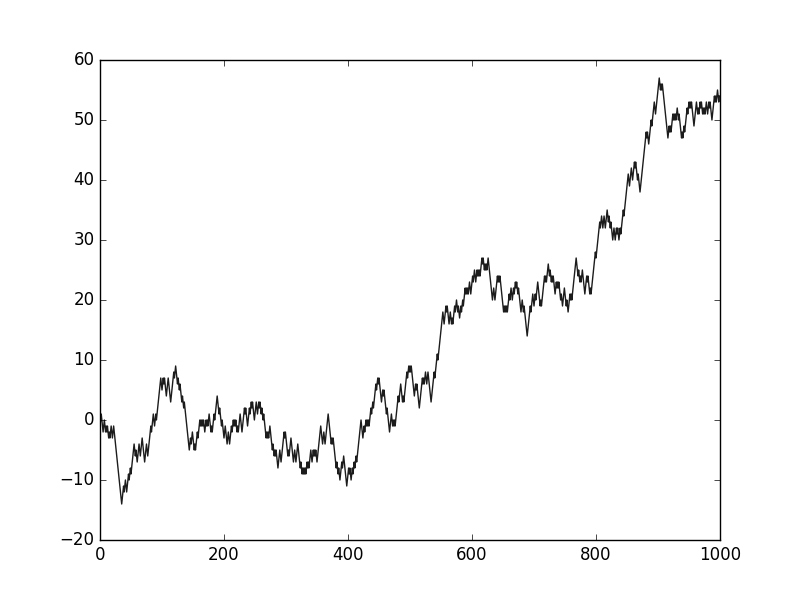
\includegraphics[scale=0.3]{img/ssrw1.png}

\example{Simple Symmetric Random Walk in $\real^2$}
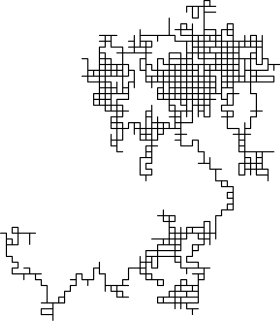
\includegraphics[scale=0.3]{img/ssrw2.png}

\definition{Brownian Motion - 1D}
Let $\mathcal{F}_t$ be a filtration.\\
\textit{Brownian Motion} is an adapted \textit{stochastic process} $W=\{W_t\}_{t\geq0}$ where
\begin{enumerate}[label=\roman*)]
	\item $W_0=x$ for some $x\in\real$.
	\item $W$ has independent and stationary Normal increments:
	\begin{enumerate}
		\item $W_{y+u}-W_t$ is independent of $\mathcal{F}_t\ \forall\ t,u\geq0$;
		\item $W_{y+u}-W_t$ \& $W_{s+u}-W_s$ has the same distribution $\forall\ s,t,u\geq 0$ with $s\leq s+u\leq t+u$;
		\item $W_{t+u}-W_t\sim N(0,u)$.
	\end{enumerate}
	\item $W$ has continuous paths \textit{i.e.} $t\mapsto W_t(\omega)$ is a continuous function of $t\ \forall\ \omega\in\Omega$.
\end{enumerate}

\definition{Standard Brownian Motion}
$W=\{W_t\}_{t\geq0}$ is said to be a \textit{Standard Brownian Motion} if $W_0=0$.\\

\proposition{Distribution of Increments of General Brownian Motion}
Let $W_t$ be \textit{Brownian Motion} with $W_t=x$ then
$$(W_t|W_0=x)\sim N(x,t)$$

\proposition{Distribution of Increments of Standard Brownian Motion}
Let $W_t$ be \textit{Standard Brownian Motion} then
$$W_t=W_t-W_0\sim N(0,t)$$

\remark{Transition Density}
\textit{Brownian Motion} has \textit{Transition Density}
$$p(t,x,y)=\frac{1}{\sqrt{2\pi t}}e^{-\frac{1}{2t}(x-y)^2}$$
where $\prob(W_t\in(y,y+\Delta y)|W_0=x)=p(t,x,y)\Delta y+o(\Delta y)$.\\
\textit{i.e} - The probability that a \textit{Brownian Motion} starting at $x$ ends up in interval $(y,y+\Delta y)$  at time $t$ is $\approx p(t,x,y)\Delta y$.\\

\proposition{Constructing the Brownian Motion of a Simple Symmetric Random Walk}
Let $Y_t$ be a simple symmetric random walk \& $S_n=\sum_{i=0}^nY_i$, assuming $S_0=0$.\\
Each step $Y_i$ has mean $0$ \& variance $1$ thus by the central limit theorem $\frac{1}{\sqrt{n}}S_n$ converges to $N(0,1)$ distribution.\\
Compressing both time \& space results in a process that converges to \textit{Brownian Motion}.\\
Define $X^n=\{X_t^n\}_{t\in[0,1]}$ by setting $X_t^n=\frac{1}{\sqrt{n}}S_{nt}\ \forall\ t=\frac{j}{n}$ and use linear interpolation in between.\\
Then $X^n$ converges to Brownian Motion.\\

\example{Expected Position of Brownian Motion}
Suppose a particle is at position $1.7$ at time $t=2$. What is the expected position at time $t=4$?
\[\begin{array}{rcl}
\expect(W_4|W_2=1.7)&=&\expect(W_4-W_2+W_2-W_0|W_2=1.7)\\
&=&\expect(W_4-W_2|W_2=1.7)+\expect(W_2-W_0|W_2=1.7)\\
&=&\expect(W_4-W_2)+1.7\\
&=&0+1.7 = 1.7
\end{array}\]

\example{Probability of Position of Brownian Motion}
Suppose the price of a produce moves according to $X_t=\sigma W_t+\mu t$ with $\sigma^2=4$ \& $\mu=-5$.\\
Given that $X_8=4$ what is the probability that the price is below 1 at time 9?
\[\begin{array}{rcl}
\prob(X_9<1|X_8=4)&=&\prob(X_9-X_8<-3|X_8=4)\\
&=&\prob(X_9-X_8<-3\\
&=&\prob(X_1=X_0<-3)\\
&=&\prob(X_1<-3)\\
&=&\prob(2W_1-5\times1<-3)\\
&=&\prob(W_1<1\\
&=&\Phi(1)\\
&=&0.8413
\end{array}\]

\subsection{Properties of Brownian Motion}

\proposition{Properties of Standard Brownian Motion}
Let $W$ be a \textit{Standard Brownian Motion} then
\begin{enumerate}[label=\roman*)]
	\item $\forall\ t\geq0,\ \expect(W_t)=0$ \& $Var(W_t)=t$;
	\item $\forall\ 0\leq s\leq t,\ Cov(W_s,W_t)=s$;
	\item $-W_t$ is a \textit{Standard Brownian Motion};
	\item For a fixed $s>0$ the process $X=\{X_t\}_{t\geq0}$ defined by $X_t=W_{t+s}-W_s$ is also a \textit{Standard Brownian Motion};
	\item For any $\alpha>0$ the process $Y=\{Y_t\}_{t\geq0}$ defined by $Y_t=\frac{1}{\sqrt{\alpha}}W_{\alpha t}$ is a \textit{Standard Brownian Motion}.
\end{enumerate}
\nb - $v)$ is known as the \textit{Scaling Property}.\\

\proof{Proposition 5.4}
\begin{enumerate}[label=\roman*)]
	\item Since $W_t\sim N(0,t)$ then $\expect(W_t)=0$ \& $Var(W_t)=t$;
	\item Let $0\leq s\leq t$ then
	\[\begin{array}{rcl}
	Cov(W_s,W_t)&=&Cov(W_s,W_t-W_s+W_s)\\
	&=&Cov(W_s,W_t-W_s)+Cov(W_s,W_s)\\
	&=&0+Var(W_s)\\
	&=&s
	\end{array}\]
	\item We check $-W_t$ has the properties of \textit{Standard Brownian Motion} as defined in \textbf{Definition 5.3} \& \textbf{Definition 5.4}
	\begin{enumerate}
		\item $-W_0=-0=0$;
		\item $-W_{t+u}-(-W_t)=-(W_{t+u}-W_t)$ we know $W_{t+u}-W_t\sim N(0,u)$.\\
		So $-(W_{t+u}-W_t)\sim N(0,u)$ by symmetry of the normal distribution \& it is independent of $\mathcal{F}_t$.
		\item $-W_t$ is continuous if $W_t$ is continuous.
	\end{enumerate}
	\item We check $X_t=W_{t+s}-W_s$ has the properties of \textit{Standard Brownian Motion} as defined in \textbf{Definition 5.3} \& \textbf{Definition 5.4}
	\begin{enumerate}
		\item $X_0=W_s-W_s=0$;
		\item $X_{t+u}-X_t=(W_{t+u+s}-W_s)+(W_{t+s}-W_s)=W_{t+u+s}-W_{t+s}\sim N(0,u)$.\\
	This is independent of $\mathcal{F}_{t+s}$.
		\item $X_t$ is the difference of two continuous functions, so is continuous.
	\end{enumerate}
	\item We check $Y_t=\frac{1}{\sqrt{\alpha}}W_{\alpha t}$ has the properties of \textit{Standard Brownian Motion} as defined in \textbf{Definition 5.3} \& \textbf{Definition 5.4}
	\begin{enumerate}
		\item $Y_0=\frac{1}{\sqrt{\alpha}}W_0=\frac{1}{\sqrt{\alpha}}\times0=0$;
		\item $Y_{t+u}-Y_t=\frac{1}{\sqrt{\alpha}}(W_{\alpha(t+u)}-W_{\alpha t})$\\
		We know $W_{\alpha t+\alpha u}-W_{\alpha t}\sim N(0,au)$ so $Y_{y+\alpha}-Y_t\sim N(0,u)$.\\
		For $t_1\leq t_2\leq t_3\leq t_4\implies \alpha t_1\leq\alpha t_2\leq\alpha t_3\leq\alpha t_4$.\\
		$Y_{t_2}-Y_{t_1}=\frac{1}{\sqrt{\alpha}}(W_{\alpha t_2}-W_{\alpha t_1})$\\
		$Y_{t_4}-Y_{t_3}=\frac{1}{\sqrt{\alpha}}(W_{\alpha t_4}-W_{\alpha t_4})$.\\
		These are independent of each other as $W_t$ is a \textit{Brownian Motion} \& the time gaps don't overlap.
		\item $Y_t$ is continuous, since $W_t$ is continuous.
	\end{enumerate}
\end{enumerate}

\remark{Brownian Motion is not differentiable}

\definition{Gaussian Process}
A \textit{Gaussian Process} is a Continuous-Time Stochastic Process with continuous sample paths \& finite dimensional distributions that are multivariable normal.\\
A \textit{Gaussian Process} is completely determined byits mean function \& auto-covariance function.\\

\theorem{All States are Recurrent in  Standard Brownian Motion}
For a \textit{Standard Brownian Motion} $W$ we have
$$\prob\left(\sup_{t\geq0}W_t=\infty,\inf_{t\geq0}W_t=-\infty\right)=1$$
\nb This implies that \textit{Brownian Motion} is recurrent.\\

\subsection{The Reflection Principle \& First Passage Time}

\theorem{The Reflection Principle}
Let $\tau_a$ be the first passage time of a \textit{Standard Brownian Motion}, $W_t$ and define
$$\widetilde{W}_t=\begin{cases}W_T&for\ t\leq\tau\\a-(W_t-a)=2a-W_t&for\ t>\tau\end{cases}$$
Then $\widetilde{W}_t$ is also a \textit{Standard Brownian Motion}.\\

\theorem{Density of First Passage Time}
The density of $\tau_a$ is given by
$$\frac{|a|}{\sqrt{2\pi t^3}}e^{-\frac{a^2}{2t}},\ t\geq0$$

\proof{Theorem 5.6}
Let $\>0$.\\
First, observe that $\{\tau_a\leq T\}=\{\sup_{0\leq t\leq T}W_t\geq a\}$.\\
Indeed, if $\tau_a\leq T$, this means the process hit $a$ by time $T$.\\
This implies that $\sup_{0\leq t\leq T}W_t$ is at least $a$ by continuity of the process.\\
On the other hand, if $\sup_{0\leq t\leq T}W_t\geq a$, this imples that the process hit $a$ for the first time by $T$.\\
By continuity
\[\begin{array}{rcl}
\prob(\tau_a\geq T)&=&\prob(\sup_{0\leq t\leq T}W_t\geq a)\\
&=&\prob(\sup_{0\leq t\leq T}W_t\geq a,W_t>a)+\prob(\sup_{0\leq t\leq T}W_t\geq a,W_t<a)\\
&=&\prob(\sup_{0\leq t\leq T}W_t\geq a,W_t>a)+\prob(\sup_{0\leq t\leq T}\widetilde{W}_t\geq a,\widetilde{W}_t>a)\\
&=&\prob(\sup_{0\leq t\leq T}W_t\geq a,W_t>a)+\prob(\sup_{0\leq t\leq T}\widetilde{W}_t\geq a,W_t>a)\mathrm{Since\ }\widetilde{W}_t\ \mathrm{is\ S.\ Brownian\ Motion}\\
&=&2\prob(\sup_{0\leq t\leq T}W_t\geq a,W_t>a)\\
&=&2\prob(W_t>a)\\
^{[1]}&=&{\displaystyle2\int_{a}^\infty\frac{1}{\sqrt{2\pi T}}e^{-\frac{1}{2t}x^2}dx}\\
&=&{\displaystyle\int_0^T\sqrt{\dfrac{a^2}{2\pi u^3}}e^{-\frac{a^2}{2u}}du}\\
\implies f_{\tau_a}(T)&=&\sqrt{\dfrac{a^2}{2\pi T^3}}e^{-\frac{a^2}{2t}}
\end{array}\]
$[1]$ consider the following substitution
\[\begin{array}{rrcl}
\mathrm{Set}&u&=&\dfrac{a^2T}{x^2}\\
\implies&du&=&-\dfrac{2a^2T}{x^3}dx\\
\&&x^6&=&\dfrac{a^6T^3}{u^3}
\end{array}\]

\theorem{For any fixed $a\neq0$ we have $\expect(\tau_a)=\infty$}

\proof{Theorem 5.7}
We only prove this for $a>0$.\\
We compute $\expect(\tau_a)$ using the standard trick of integrating the tail
$$\expect(\tau_a)=\int_0^\infty\prob(\tau_a>t)dt=\int_0^\infty\left(1-\frac{2}{\sqrt{2\pi t}}\int_a^\infty ext(-x^2/2t)dx\right)dt$$
Using the formula for $\prob(\tau_a>t)$ we have found in the previous truth.\\
But
\[\begin{array}{rcl}
{\displaystyle1-\frac{2}{\sqrt{2\pi t}}\int_a^\infty ext(-x^2/2t)dx}&=&{\displaystyle\frac{2}{\sqrt{2\pi t}}\int_0^aexp(-x^2/2t)dx}\\
\mathrm{Let}\ y=x/\sqrt{t}\implies&=&{\displaystyle\frac{2}{\sqrt{2\pi}}\int_0^{a/\sqrt{t}}exp(-y^2/2)dy}\\
\end{array}\]
Plugging into the formula for $\expect(\tau_a)$ we obtain
\[\begin{array}{rcl}
\expect(\tau_a)&=&{\displaystyle\frac{2}{\sqrt{2\pi}}\int_0^\infty\int_0^{a/\sqrt{t}}e^{-y^2/2}dy\ dt}\\
&=&{\displaystyle\frac{2}{\sqrt{2\pi}}\int_0^\infty\int_0^{a^2/y^2}e^{-y^2/2}dy\ dy}\\
&=&{\displaystyle\frac{2a^2}{\sqrt{2\pi}}\int_0^\infty\frac{1}{y^2}e^{-y^2/2}dy}\\
&\geq&{\displaystyle\frac{2a^2}{\sqrt{2\pi}}\int_0^1\frac{1}{y^2}e^{-y^2/2}dy}\\
&\geq&{\displaystyle c\frac{2a^2}{\sqrt{2\pi}}\int_0^1\frac{1}{y^2}dy}\\
&=&\infty
\end{array}\]

\subsection{Martingales}

\definition{Discrete-Time Martingale}
A stochastic process $Y=\{Y_n\}_{n\in\nats}$ is called a \textit{Discrete-Time Martingale} with respect to a filtration $\mathcal{F}_n$ if $\forall\ n\in\nats$
\begin{enumerate}[label=\roman*)]
	\item $\expect(|Y_n|)<\infty$;
	\item $\expect(Y_{n+1}|\mathcal{F}_n)=Y_n$.
\end{enumerate}

\definition{Continuous-Time Martingale}
A stochastic process $Y=\{Y_t\}_{t\geq0}$ is called a \textit{Continuous-Time Martingale} with respect to a filtration $\mathcal{F}_n$ if $\forall\ t\geq s\geq0$
\begin{enumerate}[label=\roman*)]
	\item $\expect(|Y_t|)<\infty$;
	\item $\expect(Y_t|\mathcal{F}_s)=Y_s$.
\end{enumerate}

\definition{Supermartingale}
$Y=\{Y_n\}_{n\in\nats}$ is called a \textit{Supermartingale} with respect to a filtration $\mathcal{F}_n$ if $\forall\ n$
\begin{enumerate}[label=\roman*)]
	\item $\expect(|Y_n|)<\infty$;
	\item $\expect(Y_{n+1}|\mathcal{F}_n)\leq Y_n$.
\end{enumerate}
$Y=\{Y_t\}_{t\geq0}$ is called a \textit{Supermartingale} with respect to a filtration $\mathcal{F}_n$ if $\forall\ n$
\begin{enumerate}[label=\roman*)]
	\item $\expect(|Y_n|)<\infty$;
	\item $\expect(Y_{n+1}|\mathcal{F}_n)\geq Y_n$.
\end{enumerate}

\remark{Common Filtrations}
Often $\mathcal{F}_n$ or $\mathcal{F}_t$ are taken to be the filtration generated by the process itself, $\{Y_n:n\in\nats\}$ or $\{Y_s:0\leq s\leq t\}$.\\

\remark{Iterated Expectation of Martingale}
By the \textit{Law of Iterated Expectation}
$$\expect(Y_{n+1})=\expect(\expect(Y_{n+1}|\mathcal{F}_n))=\expect(Y_n)\ \forall\ n\in\nats$$
\nb For \textit{supermartingales} replace $=$ with $\leq$ \& $\geq$ respectively.\\

\example{Simple Symmetric Random Walk is a Martingale}
Let $X_1,X_2,\dots$ be IID random variables with $\prob(X_i=1)=\prob(X_i=-1)=\frac{1}{2}$.\\
Fixing $k$ let $Y_0=k$ and for $n\geq 1$ define $Y_n=k+X_1+\dots+X_n$.\\
Then $\{Y_n\}_{n\in\nats}$ is a simple symmetric random walk which starts at $k$.\\
Let $\mathcal{F}_n=\sigma(X_1,\dots,X_n)$.
\[\begin{array}{rcl}
\expect(|Y_n|)&=&\expect(|k+X_1+\dots+X_n|)\\
&\leq&\expect(|k|)+\expect(|X_1|)+\dots+\expect(|X_n|)\\
&=&|k|+n\expect(X_1)\\
&=&|k|+n\\
&<&\infty\ \forall\ n\in\nats\\
\expect(Y_{n+1}|\mathcal{F}_n)&=&\expect(Y_n+Y_{n+1}|\mathcal{F}_n)\\
&=&\expect(Y_n|\mathcal{F}_n)+\expect(X_{n+1}|\mathcal{F}_n)\\
&=&Y_n+\expect(X_{n+1})\\
&=&Y_n
\end{array}\]
Thus  $Y_n$ is a martingale.\\

\definition{Stopping Time of Filtration}
Let $X$ be a stochastic process with the associated filtration $\mathcal{F}_n$ (or $\mathcal{F}_t$).\\
Then $T$ is said to be a \textit{Stopping Time of $\mathcal{F}_n$} (or $\mathcal{F}_t$) if for every $k$ (or $s$) the event $\{T\leq k\}$ (or $\{T\leq s\}$) if $\mathcal{F}_k$-measurable (or $\mathcal{F}_s$-measurable).\\
\nb Stopped martingales are still martingales.\\

\theorem{Stopped Discrete-Time Martingale}
Let $Y=\{T_n\}_{n\in\nats}$ be a \textit{super-martingale} with respect to $\mathcal{F}_n$ and let $T$ be a stopped time.\\
Then $Z=\{Z_n\}_{n\in\nats}$ is defined as $Z_n=Y_{T\wedge n}=\begin{cases}Y_n&n\leq t\\Y_T&n>t\end{cases}$.\\

\proof{Theorem 5.8}
Notice that $Y_n=Y_0+\sum_{i=1}^n(Y_i-Y_{i-1})$ and $Z_n=Y_0+\sum_{i=1}^n\mathds{1}_{\{i\leq T\}}(Y_i-Y_{i-1})$. Then
\[\begin{array}{rcl}
\expect(Z_{n+1}|\mathcal{F}_n)-Z_n&=&\expect(Z_{n+1}-Z_n|\mathcal{F}_n)\\
&=&\expect(\mathds{1}_{\{n+1\leq T\}}(Y_{n+1}-Y_n)|\mathcal{F}_n)\\
&=&\mathds{1}_{\{n<T\}}\expect(Y_{n+1}-Y_n|\mathcal{F}_n)
\end{array}\]
Thus $Z_n$ is a supermartingale.\\

\theorem{Optional Stopping Theorem - Discrete Time}
Let $Y=\{Y_n)_{n\in\nats}$ be a discrete-time martingale with respect to $\mathcal{F}_n$ and let $T$ be a stopping time of $\mathcal{F}_n$.\\
If any of the following holds then $\expect(Y_T)=\expect(Y_0)$.
\begin{enumerate}[label=\roman*)]
	\item $T$ is (almost surely) bounded - $\exists K\in\real^+\ st\ \prob(T<K)=1$.
	\item $T$ is (almost surely) finite and $\exists\ K>0$ st $|Y_{T\wedge n}|<K\ \forall\ n\geq0$.
	\item $\expect(T)<\infty$ \& $\exists\ K\in\real^+\ st\ |Y_n-Y_{n-1}|\leq K\ \forall\ n<T$.
	\item $T$ is (almost surely) finite and $\expect(|Y_T|)<\infty$ \& $\expect(Y_n\mathds{1}_{\{T>n\}}\to0$ as $n\to\infty$.
\end{enumerate}

\theorem{Martingale Convergence Theorem - Discrete Time}
Let $Y=\{Y_n\}_{n\in\nats}$ be a supermartingale wrt $\mathcal{F}_n$.\\
Suppose $\exists\ A>0$ st $\expect(|Y_n|)\leq A\ \forall\ n\in\nats$.\\
Then $\exists$ a random variable $Y_\infty$ st
$$\prob\left(\lim_{n\in\infty}Y_n=Y_\infty\right)=1$$
\textit{i.e} For almost every $\omega$, $lim_{n\to\infty}Y_n(\omega)=Y_\infty(\omega)$ or $\lim_{n\to\infty}Y+n=Y_\infty$.\\

\theorem{Existsnce of $Z_\infty$}
If $Z_n$ is a non-negative supermartingale wrt $\mathcal{F}_n$ then $\exists$ a random variable $Z_\infty$ st $Z_n\to Z_\infty$.\\

\proof{Theorem 5.11}
\[\begin{array}{rcl}
\expect(|Z_n|)&=&\expect(Z_n)\ \mathrm{as}\ Z_n\geq0\\
&=&\expect(\expect(Z_n|\mathcal{F}_{n-1}))\\
&\leq&\expect(Z_{n-1})\ \mathrm{since}\ Z_n\ mathrm{is\ a\ supermartingale}\\
&\leq&\expect(Z_0)\\
&<&\infty\ \mathrm{as}\ \expect(|Z_nZ)<\infty\ \forall\ n\ \mathrm{by\ definition\ of\ martingale}
\end{array}\]
It follows from \textit{Martingale Convergence Theorem} that $\exists\ Z_0$ st $Z_n\to Z_\infty$.\\

\remark{}
\textit{Standard Brownian Motion} does not satisfy the assumption in the \textit{Martingale Convergence Theorem}.\\
It may, or may not, satisfy the assumption in the \textit{Optional Stopping Theorem}.

\subsection{Application of Gambler's Ruin}

\proposition{}
Let $X_1,X_2,\dots$ be iid random variables st $\prob(X_i=1)=p$ \& $\prob(X_i=-1)=1-p=:q$.\\
Let $S_0=k$ where $1\leq k\leq N-1$ and for $n\geq 1$ set $S_n=k+X_1+\dots+X_n$.\\
Thus $\{S_n\}_{n\in\nats}$ is an unrestricted random walk starting at $k$.\\
Let $T=\min\{n:S_n=0\ \mathrm{or}\ S_n=N\}$ with $T$ taken to be $\infty$ if $1\leq S_n\leq N-1\ \forall\ n\in\nats$.\\
Let $Y_n=S_{T\wedge n}$.\\
Then $\{Y_n\}_{n\in\nats}$ is a random walk with absorbing barriers at $0$ and $N$.\\
In particular before stopping (\textit{i.e} $1\leq i\leq N-1$)
$$\prob(Y_{n+1}=i-1|Y_n=i)=q\ \prob(Y_{n+1}=i+1|Y_n=i)=p$$
Also
$$\prob(Y_{n+1}=0|Y_n=0)=1\ \prob(Y_{n+1}=N|Y_n=N)=1$$
Let $\mathcal{F}_n=\sigma(X_1,\dots,X_n)$.\\
\\
We check that $Y_n$ is a martingale wrt $\mathcal{F}_n$ if $p=q=\frac{1}{2}$.\\
Since $p=q=\frac{1}{2}$
\[\begin{array}{rrcl}
\implies&\expect(Y_{n+1}|Y_n=i)&=&i\ \forall\ i\in[1,N)\\
,&\expect(Y_{n+1}|Y_n=0)&=&0\\
\&&\expect(Y_{n+1}|Y_n=N)&=&1
\end{array}\]
Hence $\expect(Y_{n+1}|\mathcal{F}_n)=\expect(Y_{n+1}|Y_n)\ \forall\ n$ by \textit{Markov Property} \& $\expect(|Y_n|)\leq N<\infty$.\\
So $Y_n$ is a martingale.\\

\theorem{Properties of Gambler's Ruin Martingale}
Suppose $p=\frac{1}{2}=q$. then
\begin{enumerate}
	\item $\prob(T<\infty)=1$
	\item $\prob(Y_T=N)=\frac{Y_0}{N}=\frac{k}{N}$; and,
	\item $\expect(T)=Y_0(N-Y_0)=k(N-k)$.
\end{enumerate}

\Proof{Theorem 5.12}
\begin{enumerate}
	\item We know that $Y_n=S_{T\wedge n}$ is a Martingale \& $Y_n\in[0,N]\ \forall\ n\in\nats$.\\
	Hence $\expect(|Y_n|)<N+1$ so by \textit{Martingale Converge Theory} $\exists Y_\infty$ st $Y_n\to Y_\infty$ almost surely.\\
	if $T(\omega)=\infty$ then $Y_n(\omega)\in[1,N-1]\ \forall\ n\in\nats$ and $|Y_{n+1}(\omega)-Y_n(\omega)|=1$.\\
	This violates the \textit{Cauchy Criterion} for convergence, so the process $Y_n$ does not converge.\\
	So $\prob(T=\infty)\leq\prob(Y_n\ \mathrm{does\ not\ converge})=0$ by the \textit{Martingale Converge Theorem}.\\
	$\implies \prob(T<\infty)=1$.
	\item We know that $T<\infty$ as $|Y_n<N+1\ \forall\ n>0$.\\
	Hence assumption $ii)$ of the \textit{Optional Stopping Theorem} holds ($expect(Y_t)=\expect(Y_0)=k$.\\
	$\implies 0.\prob(Y_t=0)+N.\prob(Y_t=N)=k$\\
	$\implies\prob(Y_T=N)=\frac{k}{N}$.
	\item Define $Z_n:=S_n^2-n$. We have already proved this to be a Martingale.\\
	We have
	\[\begin{array}{rcl}
	\expect(T)&=&\sum_{k=1}^n\prob(T>k)\\
	&=&\sum_{r=0}^\infty\left(\prob(T>rN)+\prob(T>rN12)+\dots+\prob(T>rN+n)\right)\\
	&\leq&\sum_{r=0}^\infty n.\prob(T>rN)
	\end{array}\]
	
	\[\begin{array}{rrcl}
	\mathrm{For\ }r=1&\prob(T>N)&=&\prob(S_n\in[1,N-1],n\leq N)\\
	&&=&1-\prob(T\leq N)\\
	&&\leq&1-\prob(A)\ \mathrm{where}\ A=\{-1,+1,\dots,-1\}\subset\{T\leq N\}\\
	&&=&1-\frac{1}{2^N}\\
	\mathrm{For\ }r=2&\prob(T>2N)&=&\prob(S_n\in[1,n-1],n\leq 2N)\\
	&&=&\prob\big(S_n\in[1,N-1],n\in[1,N]\big)\\
	&&\times&\prob\big(S_n\in[1,N-1],n\in[N+1,2N]\big|S_n\in[1,N-1]\big)\\
	&&\leq&\prob(T>N)\prob(T'>N)\\
	&&=&\left(1-\frac{1}{2^N}\right)^2\\
	\mathrm{So}&\prob(T>rN)&\leq&\left(1-\frac{1}{2^N}\right)^r\ \forall\ r\in[1,N]
	\end{array}\]
	Since $\left|1-\frac{1}{2^N}\right|<1\implies\expect(T)<\infty$.\\
	Since $T$ is bounded, by the first assumption, the \textit{Optional Stopping Theorem} holds.
	Thus
	\[\begin{array}{rrcl}
	&\expect(Z_T)&=&\expect(Z_0)=S_0^2=k^2\\
	\implies&k^2&=&\expect(S_T^2-T)\\
	&&=&\expect(S_T^2)-\expect(T)\\
	&&=&0^2.\prob(S_T=0)+N^2.\prob(S_T=N)-\expect(T)\\
	&&=&N^2.\frac{k}{N}-\expect(T)\\
	\implies&\expect(T)&=&k(N-k)\\
	\&&|Z_n-Z_{n-1}|&=&|S_n^2-S_{n-1}^2+1|\\
	&&\leq&|S_n^2|+|S_{n-1}^2|+1\\
	&&\leq&2N^2+1\ \forall\ n
	\end{array}\]
\end{enumerate}

\theorem{Special Martingale}
Let $Y=\{Y_n\}_{n\in\nats}$ defined by $Y_n=k+X_0+\dots+X_n$, be the absorbed random walk on $[0,N]$ with $p\neq q$, $\mathcal{F}_n=\sigma(X_1,\dots,X_n)$.\\
Let $V_n=(q/p)^{Y_n}$, then $\{V_n\}_{n\in\nats}$ is a \textit{Martingale} wrt $\mathcal{F}_n$.\\

\proof{Theorem 5.13}
Since $Y_n\in[0,N]$ then
$$\expect(|V_n|)=\expect(V_n)=\expect\left(\left(\frac{q}{p}\right)^{Y_n}\right)\leq\max\left\{\left(\frac{q}{p}\right)^0,\left(\frac{q}{p}\right)^N\right\}<\infty$$
\[\begin{array}{rcl}
\expect(V_{n+1}|\mathcal{F}_n)&=&\expect\left(\left(\frac{q}{p}\right)^{Y_{n+1}}|\mathcal{F}_n\right)\\
&=&\expect\left(\left(\frac{q}{p}\right)^{Y_n+1}|Y_n\right)\mathrm{\ by\ Markov\ Property}\\
\expect(V_{n+1}|Y_n=0)&=&\left(\frac{q}{p}\right)^0=\left(\frac{q}{p}\right)^{Y_1}=V_n\\
\expect(V_{n+1}|Y_n=N)&=&\left(\frac{q}{p}\right)^N=\left(\frac{q}{p}\right)^{Y_n}=V_n\\
\mathrm{For}\ i\in[1,N-1]\\
\expect\left(\left(\frac{q}{p}\right)^{Y_{n+1}}|Y_n=i\right)&=&\left(\frac{q}{p}\right)^{i=1}p+\left(\frac{q}{p}\right)^{i-1}q\\
&=&\left(\frac{q}{p}\right)^i[q+p]\\
&=&\left(\frac{q}{p}\right)^i\times1\\
&=&V_n
\end{array}\]
$V_n$ is a martingale.\\

\theorem{Properties from Theorem 5.13}
Let $Y$ be as in previous lemma. Let $T$ be the first time $Y$ hits $0$ or $N$. Then
\begin{enumerate}
	\item $\prob(T<\infty)=1$; and,
	\item $\prob(Y_T=N)=\dfrac{1-(q/p)^k}{1-(q/p)^N}$
\end{enumerate}

\proof{Theorem 5.14}
\begin{enumerate}
	\item Let $V_n=V_n=\left(\frac{q}{p}\right)^{Y_n}$.\\
	Then $V_n$ is a martingale \& $V_n\leq\max\left\{\left(\frac{q}{p}\right)^0,\left(\frac{q}{p}\right)^N\right\}$.\\
	By the \textit{Martingale Convergence Theorem} we know $V_n$ converges, almost surely, to some $V_\infty$.\\
	Now, $\{T=\infty\}=\left\{V_n\subset\left\{\left(\frac{q}{p}\right)^1,\dots,\left(\frac{q}{p}\right)^{N-1}\right\}\ \forall\ n>0\right\}$.\\
	So $\exists\ \delta>0$ st $|V_{n+1}-V_n|>\delta\ \forall\ n$ which implies that $V_n$ does not converge.\\
	So $P(T=\infty)=\prob\left(V_n\subset\left\{\left(\frac{q}{p}\right)^1,\dots,\left(\frac{q}{p}\right)^{N-1}\right\}\ \forall\ n>0\right)\leq\prob(V_n\ \mathrm{does\ not\ converge})=0$ by \textit{Martingale Convergence Theorem}.
	\item Since $T<\infty$ almost surely, by $1)$, and $\forall\ n\leq\max\left\{\left(\frac{q}{p}\right)^0,\left(\frac{q}{p}\right)^N\right\}$ then condition $iii)$ of \textit{Optional Stopping Distance} holds.
	\[\begin{array}{rrcl}
	\implies&\expect(V_t)&=&\expect(V_0)=\left(\frac{q}{p}\right)^k\\
	\implies&\left(\frac{q}{p}\right)^0\prob(Y_t=0)+\left(\frac{q}{p}\right)^N\prob(Y_T=N)&=&\left(\frac{q}{p}\right)^k\\
	\implies&1\times\left(1-\prob(Y_T=N)\right)+\left(\frac{q}{p}\right)^N\prob(Y_T=N)&=&\\
	\implies&\prob(Y_T=n)&=&\dfrac{1-\left(\frac{q}{p}\right)^k}{1-\left(\frac{q}{p}\right)^N}
	\end{array}\]
\end{enumerate}

\subsection{Brownian Motion as a Martingale}

\theorem{Standard Brownian Motion as a Martingale}
Let $\{W_t\}_{t\geq0}$ is \textit{Standard Brownian Motion} with filtration $\mathcal{F}_t$ generated by the process itself, then
\begin{enumerate}[label=\arabic*)]
	\item $W_t$ is a martingale.
	\item $W_t^2-t$ is a martingale.
	\item $X_t=at+\sigma W_t$ is a martingale iff $a=0$.
	\item $Y_t=e^{at+\sigma W_t}$ is a martingale iff $a=-\frac{\sigma^2}{2}$.
\end{enumerate}

\proof{Theorem 5.15}
\begin{itemize}
	\item[3)] Let $X_t=at+\sigma W_t$.
		\[\begin{array}{rcl}
		\expect(|X_t|)&=&\expect(|at+\sigma W_t|)\\
		&\leq&\expect(|at|)+\expect(|\sigma W_t|)\\
		&=&|at|+\sigma\expect(|W_t|)\\
		&\leq&t|a|+\sigma\expect(W_t^2)^{1/2}\\
		&=&t|a|+\sigma t\\
		&<&\infty\ \forall\ t>0\\
		\mathrm{Let}\ 0\leq s\leq t\\
		\expect(X_t|\mathcal{F}_s)&=&\expect(at+\sigma W_t|\mathcal{F}_s)\\
		&=&at+\sigma\expect(W_t-W_s+W_s|\mathcal{F}_s)\\
		&=&at+\sigma\expect(W_t-W_s)+\sigma W_s\\
		&=&at+\sigma\times0+\sigma W_s\\
		&=&at+\sigma W_s
		\end{array}\]
		We want $\expect(X_t|\mathcal{F}_s)=X_s$.Set
		\[\begin{array}{rrcl}
		&as+\sigma W_s&=&at+\sigma W_s\\
		\implies& a(s-t)&=&0\\
		\implies& a&=&0
		\end{array}\]
	\item[4)]Let $Y_t=e^{at+\sigma W_t}$.
	\[\begin{array}{rcl}
	\expect(|Y_t|)=\expect(e^{at+\sigma W_t})\\
	&=&e^{at}\expect(e^{\sigma W_t})\\
	&=&e^{at}e^{0\times\sigma+\frac{1}{2}t^2\sigma^2}\mathrm{\ by\ moment-generating\ funciton}\\
	&=&e^{at+\frac{1}{2}\sigma^2t^2}\\
	&<&\infty\ \forall\ t>0\\
	\mathrm{Let}\ 0\leq s\leq t\\
	\expect(Y_t|\mathcal{F}_s)&=&\expect(e^{at+\sigma W_t}|\mathcal{F}_s)\\
	&=&e^{at}\expect(e^{\sigma W_t}|\mathcal{F}_s)\\
	&=&e^{at}\expect(e^{\sigma(W_t-W_s+W_s)}|\mathcal{F}_s)\\
	&=&e^{at+\sigma W_s}\expect(e^{\sigma(W_t-W_s)})\\
	&=&e^{at+\sigma W_s}e^{0+\frac{1}{2}\sigma^2(t-s)}\\
	&=&e^{at+\sigma W_s+\frac{1}{2}\sigma^2(t-s)}
	\end{array}\]
	Setting $\expect(Y_t|\mathcal{F}_s)$ yields that $a=-\frac{\sigma^2}{2}$.
\end{itemize}

\proposition{Stopping Time of Brownian Motion}
Let $a,b>0$ and $\tau=\min\{t\geq0:W_t\in\{a,-b\}\}$. Then
$$\prob(W_\tau=a)=\frac{b}{a+b}\ \mathrm{and}\ \expect(\tau)=ab$$

\proof{Proposition 5.6}
We know that $\expect(\tau)<\infty$, almost surely.\\
If we define $Z:=\max\{a,b\}$ then $|W_{t\wedge\tau}|\leq Z$.\\
Then the \textit{Optional Stopping Theorem} holds (\textit{i.e.} $\expect(W_\tau)=\expect(W_0)=0$.
\[\begin{array}{rrcl}
\implies&a\prob(W_\tau=a)+(-b)\prob(W_\tau=-b)&=&0\\
\implies&a\prob(W_\tau=a)+(-b)(1-\prob(W_\tau=a))&=&0\\
\implies&\prob(W_\tau=a)&=&\dfrac{b}{a+b}
\end{array}\]

\proposition{Which Absorbing Barrier is Hit}
Let $X_t=\mu t+\sigma W_t$ with $\mu<0$ \& $M=\max\{X_t:t\geq0\}$.\\
For $a,b>0$
$$\prob(\tau_a>\tau_{-b})=\frac{1-e^{-\alpha b}}{e^{\alpha a}-e^{-\alpha b}}\ \mathrm{with}\ \alpha=-\frac{2\mu}{\sigma^2}$$
Thus
$$\prob(M\geq a)=e^{-\alpha a}$$

\proof{Proposition 5.7}
First we prove that $e^{\alpha X_t}$ is a \textit{Martingale}.
\[\begin{array}{rcl}
\expect(|e^{alpha X_t}|)&=&\expect(e^{\alpha X_t})\\
&=&\expect(e^{\alpha\mu t+\sigma\alpha W_t})\\
&=&e^{\alpha\mu t}\expect(e^{\sigma\alpha W_t})\\
&=&e^{\alpha\mu t}e^{0+\frac{1}{2}\sigma^2\alpha^2t}\\
&<&\infty\ \forall\ t>0\\
\mathrm{Let\ }0\leq s<t\\
\expect(e^{\alpha X_t}|\mathcal{F}_s)&=&\expect(e^{\alpha\mu t+\alpha\sigma W_t}|\mathcal{F}_s)\\
&=&e^{\alpha\mu t}\expect)e^{\alpha\sigma(W_t-W_s+W_s)}|\mathcal{F}_s)\\
&=&e^{\alpha\mu t+\alpha\sigma W_s}\expect(e^{\alpha\sigma(W_t-W_s)})\\
&=&e^{\alpha\mu t+\alpha\sigma W_s}e^{\frac{1}{2}\alpha^2\sigma^2(t-s)}\\
\mathrm{Setting}\ \alpha=-\frac{2\mu}{\sigma^2}\\
\expect(e^{\alpha W_t}|\mathcal{F}_s)&=&e^{-2\frac{\mu^2t}{\sigma^2}-2\frac{\mu W_s}{\sigma}+\left(4\frac{\mu^2}{\sigma^2}\right)\left(\frac{t-s}{2}\right)}\\
&=&e^{-2\frac{\mu}{\sigma^2}(\mu s+\sigma W_s)}\\
&=&e^{\alpha X_s}
\end{array}\]


\newpage
\setcounter{section}{-1}
\section{Reference}

\subsection{Notation}

\notation{Collection of Events}
A collection of events are denoted by $\mathcal{C}$.\\

\notation{Infimum}
Let $S$ be a subset of an ordered set $T$.\\
The \textit{Infimum} of $S$ is the greatest element in $T$ that is less of equal to all elements of $S$.\\
This is denoted by
$$\inf(A)$$

\notation{Minimum}
$$x\wedge y:=\min(x,y)$$

\notation{Poisson Process}
A \textit{Poisson Process} is denoted by $\{N_t\}_{t\geq 0}$.\\
Individual events in this sequence are denoted by $N_i$.\\

\notation{Power Set}
The power set of set $S$ is denoted by $2^S\ or\ \{0,1\}^S$.\\

\notation{Sample Space}
The \textit{Sample Space} of a variable is denoted by $\Omega$.\\

\notation{Transition}
A transition between state $x$ \& $y$ is generally denoted by $p_{xy}$.\\

\subsection{Definitions}

\definition{Convex \& Concave Functions}
A \textit{Convex Function} is a continuous function whose value at the midpoint of every interval in its domain does not exceed the arithmetic mean of its values at the ends of the interval.\\
A \textit{Concave Function} whose value at the midpoint of every interval in its domain exceeds teh arithmetic mean of its values at the ends of the interval.\\
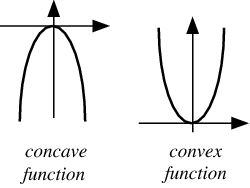
\includegraphics[scale=0.5]{img/convexConcave.png}

\definition{Co-Variance}
\textit{Co-Variance} is a measure of the joint variability of two random variables.\\
A greater magnitude of \textit{Co-Variance} corresponds to the two variables having similar behaviour.\\
A positive \textit{Co-Variance} means that as one variable increases when the other tends to.\\
A negative \textit{Co-Variance} means that as one variable decreases when the other tends to increase.\\
$$Cov(X,Y)=\expect\left((X-\expect(X)(Y-\expect(Y)\right)$$

\definition{Index Set}
An \textit{Index Set} is a set whose members are used to index members of another set.\\

\definition{Indicator Function}
The \textit{Indicator Function} of an event returns $1$ or $0$ to denote whether a given event event occurs
$$1_A(\omega)=\begin{cases}1&w\in A\\0&\omega\not\in A\end{cases}$$

\definition{Moment Generating Function}
For random variable $X$ with probability mass function $p_X(k)$ has a \textit{Moment Generating Function}
$$m_X(\theta)=\expect(e^{\theta X})=\sum_k p_x(k)e^{\theta k}$$

\definition{Probability Generating Function}
For random variable $X$ with probability mass function $p_X(k)$ has a \textit{Probability Generating Function}
$$P_X(s)=\expect(s^X)=\sum_Kp_X(k)s^k$$

\definition{Right-Continuous Function}
A \textit{Right-Continuous Function} is one in which no jump occurs when the limit point is approached from the right hand size.\\

\definition{Unitary Matrix}
$P$ is a \textit{Unitary Matrix} if $P^{-1}=P^*$ where $P^*$ is the hermitian matrix of $P$.

\subsection{Theorems}

\theorem{Cauchy Criterion for Convergence}
A sequence $\{a_n\}$ converges iff
$$\forall\ \varepsilon>0\ \exists N\in\nats\ st\ \forall\ m,n\in\nats\ \mathrm{with}\ m,n>N\ |a_m-a_n|<\varepsilon$$

\theorem{Cauchy-Schwarz Inequality}
Let $X$ \& $Y$ be random variables with finite variance, then
$$\expect(|XY|)\leq\sqrt{\expect(X^2)\expect(Y^2)}$$

\theorem{Conditional Probability}
$$\prob(A|B)=\dfrac{\prob(A\bigcap B)}{\prob(B)}$$

\theorem{Covariance Identities}
The following are identities concerning the \textit{Covariance}
\[\begin{array}{rcl}
Cov(X+Y)&=&\expect(XY)-\expect(X)+\expect(Y)\\
Cov(X,a)&=&0\\
Cov(X,aY)&=&aCov(X,Y)\\
Cov(X,Y+Z)&=&Cov(X,Y)+Cov(X,Z)
\end{array}\]

\theorem{Expectation of Expectation of Conditional}
$$\expect(\expect(Y|X))=\expect(Y)$$

\theorem{Expected Value of Indicator Function}
$$\expect(1_A)=\prob(A)$$

\theorem{Jensen's Inequality}
If $g$ is a convex function, then
$$\expect(g(X))\geq g(\expect(X))$$
If $g$ is a concave function, then
$$\expect(g(X))\leq g(\expect(X))$$
\theorem{L'H\^{o}pitals Rule}
If $\lim_{x\to a}\frac{f(x)}{g(x)}=\frac{0}{0}$or$=\frac{\infty}{\infty}$ then
$$\lim_{x\to a}\frac{f(x)}{g(x)}=\lim_{x\to a}\frac{f'(x)}{g'(x)}$$

\theorem{Markov's Inequality}
Let $X$ be a non-negative random variable, then $\forall c>0$
$$\prob(X>c)\leq\frac{\expect(X)}{c}$$

\theorem{Probability of Event as Integral}
$$\prob(x\in A)=\int_y\prob(x\in A|Y=y)F_Y(y)dy$$

\theorem{Stirling's Formula}
For $n\in\nats$
$$n!~\sqrt{2\pi n}\left(\frac{n}{e}\right)^n\ \mathrm{as}\ n\rightarrow\infty$$

\theorem{Sum of Exponentials}
Let $X_1,\dots,N_n\sim Exp(\lambda)$. Then
$$X_1+\dots+X_n\sim\Gamma(b,\lambda)$$

\subsection{Probability Distributions}

\definition{Binomial Distribution}
Let $X$ be a discrete random variable modelled by a \textit{Binomial Distribution} with $n$ events and rate of success $p$.\\
\[\begin{array}{rcl}
p_X(k)&=&{n\choose k}p^k(1-p)^{n-k}\\
\expect(X)np=&\&&Var(X)=np(1-p)
\end{array}\]

\definition{Gamma Distribution}
Let $T$ be a continuous randmo variable modelled by a \textit{Gamma Distribution} with shape parameter $\alpha$ \& scale parameter $\lambda$. Then
\[\begin{array}{rcll}
f_T(x)&=&\dfrac{\lambda^\alpha x^{\alpha-1}e^{-\lambda x}}{\Gamma(\alpha)}&\mathrm{for\ }x>0\\
\expect(T)=\dfrac{\alpha}{\lambda}&\&&Var(T)=\dfrac{\alpha}{\lambda^2}
\end{array}\]
\nb $\alpha,\lambda>0$.\\

\definition{Exponential Distribution}
Let $T$ be a continuous random variable modelled by a \textit{Exponential Distribution} with parameter $\lambda$. Then
\[\begin{array}{rcll}
f_T(t)&=&\lambda e^{-\lambda t}&\mathrm{for\ }t>0\\
F_T(t)&=&1-e^{-\lambda t}&\mathrm{for\ }t>0\\
\expect(X)=\frac{1}{\lambda}&\&&Var(X)=\frac{1}{\lambda^2}
\end{array}\]
\nb Exponential Distribution is used to model the wait time between decays of a radioactive source.\\

\definition{Normal Distribution}
Let $X$ be a continuous random variable modelled by a \textit{Normal Distribution} with mean $\mu$ \& variance $\sigma^2$.\\
Then
\[\begin{array}{rcl}
f_X(x)&=&\dfrac{1}{\sqrt{2\pi\sigma^2}}e^{-\frac{(x-\mu)^2}{2\sigma^2}}\\
F_X(x)&=&\dfrac{1}{\sqrt{2\pi\sigma^2}}\int\limits_{-\infty}^xe^{-\frac{(y-\mu)^2}{2\sigma^2}}dy\\
M_X(\theta)&=&e^{\mu\theta+\sigma^2\theta^2(1/2)}\\
\expect(X)=\mu&\&&Var(X)=\sigma^2
\end{array}\]

\definition{Poisson Distribution}
Let $X$ be a discrete random variable modelled by a \textit{Poisson Distribution} with parameter $\lambda$. Then
\[\begin{array}{rcll}
p_X(k)&=&\frac{e^{-\lambda}\lambda^k}{k!}&\mathrm{For\ }k\in\nats_0\\
\expect(X)=\lambda&\&&Var(X)=\lambda
\end{array}\]
\nb Poisson Distribution is used to model the number of radioactive decays in a time period.\\

\end{document}
